\chapter{Korelační analýza}
\label{ch:korelacnianalyza}
Tato kapitola se věnuje popisu korelační analýzy pro zjištění důvodu shrinků produktů. Tuto analýzu je možné spustit na data libovolné společnosti, pokud obsahují vstupy, které jsou definované dále. Analýza byla napsána v~jazyce Python, jako sada funkcí sdružená do modulu. Ukázka volání funkcí pro spuštění analýzy je pak vytvořená v~Jupyter Notebooku. V~této kapitole je popsána implementace funkcí a princip analýzy. 

Na základě analýz dat popsaným v sekcích \ref*{sec:priprava}, \ref*{sec:vizualizace:vysl}, \ref*{sec:hypo} nebyl nalezen jednoznačný ukazatel, který by umožnil obecně charakterizovat příčiny vzniku shrinků pouze ze záznamů o jednom produktu. Proto vznikla myšlenka porovnávat zaznamenaný shrink  jednoho produktu s~jinými produkty, konkrétně s~ jejich začleněním do promoakcí v~ daném období a s~tržbami. 
Další analýza proto hodnotí korelaci mezi hodnotou shrinku a tržbami. Na základě získaných výsledků roztřídí produkty ve vstupních datech do několika kategorií, podle toho jaký vliv na ně mají ostatní produkty.

Je důležité mít na paměti, že korelace neznamená kauzalitu. Avšak z~ businessového pohledu na zkoumanou situaci si dovolíme předpokládat, že z~ hodnot korelace mezi sledovanými veličinami lze vyvodit alespoň částečnou příčinu vzniku shrinku produktu.

Pro účely této analýzy bylo potřeba získat z~ databáze tabulku týkající se všech prodejů za měsíc březen roku 2023 bez agregace na prodejny nebo části měsíce. 

% Je možné specifikovat úroveň kategorie, na které se analýza spočítá. Dále je třeba určit konkrétní název kategorie.

% https://mathstat.econ.muni.cz/media/12657/pear_cor.pdf
% https://is.muni.cz/www/98951/41610771/43823411/43823458/44159634/44707073/Pavlik_-_Biostatistika_-_kapitola_11.pdf

% úrovně 4, neboť nižší kategorie ve většině případů produkty již dále nedělí, ale pouze specifikují popis kategorie na   

\section{Postup}
\label{sec:kor:postup}
V rámci analýzy se porovnávají pouze záznamy produktů, které se vyskytují ve stejné kategorii. Jedno pozorování je na agregované na produkt, prodejnu a den záznamu. Základní hypotéza je, že shrink produktu může být ovlivněn promoakcemi jiných produktů v~kategorii.

Hodnotu shrinku jsem porovnávala s~následujícími ukazateli. 
\begin{itemize}
    \itemsep0em 
    \item Tržby daného produktu.
    \item Tržby daného produktu, které byly v~daný den v~promoakci - ukázalo se, že takové, až na výjimky nejsou.
    \item Součet tržeb všech ostatních produktů v~kategorii.
    \item Součet tržeb všech ostatních produktů v~kategorii, které byly v~daný den v~promoakci.
    \item Součet tržeb všech ostatních produktů v~kategorii, které byly v~daný den v~promoakci nebo byly v~rozmezí jednoho týdne po promoakci.
\end{itemize}

Ke každému ukazateli, jsem ještě vytvořila analogický ukazatel, který uvažoval zpoždění shrinku. V~takovém ukazateli, se nebrala hodnota prodeje ze stejného dne, jako byl den záznamu shrinku, ale hodnota z~předchozího dne. Důvodem pro vytvoření takových ukazatelů byla hypotéza, že shrink se může projevit až další den po uskutečněných tržbách. 
%Důvodem může být to, že 

Na základě korelační analýzy je možné roztřídit produkty v~kategorii do šesti skupin:
\begin{itemize}
    \itemsep0em 
    \item[] \textbf{Kategorie P} - Produkty, které si samy způsobují shrink.
    \item[] \textbf{Kategorie O} - Produkty, jejichž shrink je způsoben tím, že ostatní produkty v~kategorii jsou v~promoakci.
    \item[] \textbf{Kategorie X} - Produkty, jejichž shrink se nepodařilo vysvětlit pomocí korelační analýzy.
    \item[] \textbf{Kategorie V} - Produkty, které jsou úspěšné ve výprodejích. Produkt se hodně prodává a zároveň má malé shrinky.
    \item[] \textbf{Kategorie N} - Produkty, jejichž shrink a celkové tržby (tj. vlastní i ostatních produktů) zůstávají stále v~podobném poměru, tj. pokud jsou celkově tržby vyšší je i shrink vyšší, pokud jsou obecně tržby nižší, je nižší i shrink.
    \item[] \textbf{Kategorie F} - Produkty, u nichž nebyl koeficient korelace statisticky významný.
\end{itemize}

V závislosti do které skupiny bude produkt přiřazen je poté možné říci, jak má společnost s~ takovými produkty naložit. Společnost může ovlivnit četnost a objem závozů na prodejny a také může upravit plánování promoakcí v~rámci produktových skupin. Ke snížení shrinků produktů z~kategorie P může pomoci snížit objem prodávaného množství, nebo promovat produkt s~vyšší slevou. Pro produkty zařazené jako O je navrženo doporučení zmenšit objednávané množství, když jsou produkty ze stejné kategorie v~promoakci, případně u těchto produktů dlouhodobě snížit prodejní cenu. U výprodejových produktů promoakce funguje správně, proto je pro společnost vhodné prozkoumat tyto produkty a zjistit, zda je jejich chování přenositelné i na jiné produkty. Produkty z~kategorie N jsou produkty, jejichž množství a cena byly naplánovány v~souladu s~poptávkou. Prodávané množství není doporučeno příliš snižovat, aby nedošlo k~výpadku zásob, což má za následek nespokojenost zákazníků. Nicméně pro tyto produkty by bylo vhodné najít ekologické řešení jejich odpisu, např. v~podobě potravinových bank, kompostování nebo převedení na surovinu či krmivo pro zvířata. Co se týče zbylých kategorií, je doporučeno zkoumat individuální produkty až na konkrétních lokalitách.

Na obrázku \ref*{obr:ctg:g:kategorizace1} je znázorněno rozdělení produktů vzhledem ke korelačnímu koeficientu. Kategorie jsou pro lepší orientaci na obrázku oddělené i barevně, zároveň s~popisem je u každé části i písmenné označení kategorie. 

\begin{figure}[hbtp!]
    \centering
    \captionsetup{justification=centering}
    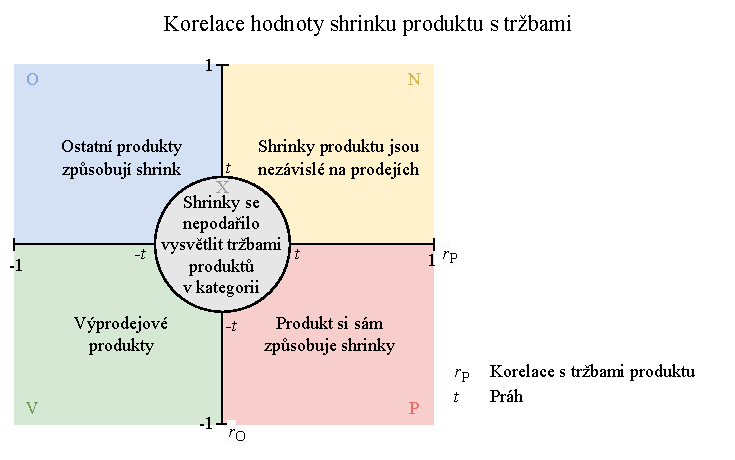
\includegraphics[width=\textwidth]{obrazky/grafy/matice_korelace_typy_DP.pdf}
    \caption{Kategorizace produktů podle korelace hodnoty shrinku s~tržbami.}
    \label{obr:ctg:g:kategorizace1}
\end{figure}

Hypotéza pro zařazení do kategorie P je následující:

Pokud je korelační koeficient zaznamenaného shrinku s~tržbami téhož produktu kladná, produkt si způsobuje shrinky sám.
Abych mohla tuto hypotézu potvrdit, nebo vyvrátit, je třeba statisticky otestovat významnost korelačního koeficientu. Formulovala jsem nulovou hypotézu $H_\mathrm{0}$ a alternativní hypotézu $H_\mathrm{A}$ pro koeficient $r_\mathrm{P}$, který měří korelaci mezi hodnotou shrinku a tržbami produktu.

\begin{equation*}
    \begin{aligned}
        H_\mathrm{0}: \quad & r_\mathrm{P} = 0 \qquad \mbox{Výběry nejsou korelované.}  \\
        H_\mathrm{A}: \quad & r_\mathrm{P} \neq 0 \qquad\mbox{Výběry jsou korelované.}\\
    \end{aligned}
\end{equation*}

Hypotéza pro zařazení do kategorie O je následující:

Pokud jsou kladně korelované hodnoty zaznamenaného shrinku a tržby ostatních produktů a zároveň korelace shrinků produktu s~vlastními tržbami je záporná, potom lze vyslovit hypotézu, že shrinky na produktu jsou způsobené ostatními produkty v~promoakci.
Pro toto tvrzení je opět nutné statisticky otestovat koeficienty korelace. Pro koeficient $r_\mathrm{P}$ je statistický test stejný jako v~předchozím případě. Pro koeficient $r_\mathrm{O}$ měřící, jak jsou korelované shrinky a tržby ostatních produktů, je třeba otestovat následující hypotézy.
\begin{equation*}
    \begin{aligned}
        H_\mathrm{0}: \quad & r_\mathrm{O} = 0 \qquad \mbox{Výběry nejsou korelované.}  \\
        H_\mathrm{A}: \quad & r_\mathrm{O} \neq 0 \qquad\mbox{Výběry jsou korelované.}\\
    \end{aligned}
\end{equation*}

Pokud na zvolené hladině významnosti zamítneme nulovou hypotézu pro zkoumané korelační koeficienty, můžeme tvrdit že s~danou pravděpodobností je koeficient statisticky významný. Na základě hodnoty korelace lze pak produkt zařadit do příslušné kategorie. Produkty, u kterých nelze zamítnout, není možné zařadit do tří uvedených kategorií.

Pro výpočet korelačního koeficientu je ještě třeba ověřit předpoklady. Pro Pearsonův korelační koeficient se jedná o~předpoklad normality dat, shodnost rozptylů a nezávislost dat. Pro Spearmanův korelační koeficient není třeba splňovat tyto předpoklady.

\section{Implementace}

V~této části je uveden přesný postup pro získání kategorizace produktů. Kód je napsaný v~jazyce Python verze 3.9. Součástí kódu je výběr kategorií, které jsou zkoumány, propojení dat shrinků, prodejů a promoakcí, výpočet korelace a ověření předpokladů, statistické testování a rozřazení produktů.

% UML diagram pro analýzu.

\subsection{Vstupy a výstupy}
\label{ss:vstupyvystupy}

Pro korelační analýzu zaznamenaných shrinků s~tržbami dalších produktů je třeba zajistit data, které se týkají zaznamenaných prodejů, produktů a~prodejen. V~násle-\\dující části jsou popsány tabulková data, která jsou nezbytná pro správné spuštění analýzy. Dále jsou definované i vstupy, které musí definovat uživatel pro specifikování názvů konkrétních sloupců v~souborech a parametry pro analýzu.

Celkem jsou požadovány čtyři vstupní tabulky - \emph{záznamy shrinků, záznamy prodejů, záznamy o~promoakcích, číselník produktů s~rozdělením produktové hierarchie}. %a~rozdělení prodejen.
Tabulka se zaznamenanými shrinky musí obsahovat sloupec s~datem záznamu, ID produktu, ID prodejny, hodnotu zaznamenaného shrinku. Tabulka s~prodeji potřebuje stejné sloupce jako tabulka se shrinky s~výjimkou že hodnota prodejů je celková prodaná částka, která byla zaznamenaná na dané prodejně v~jeden den u daného produktu. Tabulka s~údaji o promoakcích by měla obsahovat ID produktu, kterého se promoakce týká, začáteční a koncové datum promoakce a ID prodejny, pro kterou promoakce platí.
Všechny záznamové tabulky musí pokrývat stejné časové období. Období může být libovolně dlouhé.
Tabulka produktové hierarchie obsahuje ID produktu, jeho název a libovolně hluboký strom hierarchií. Každá úroveň stromu má vlastní sloupec. Všechny úrovně jsou vyplněné pro každý produkt, tato podmínka je nutná jen pro kategorie, které bude chtít uživatel využít při analýze. 
Tabulka s~hierarchií produktů slouží k~tomu, aby mohla být napojena na ostatní tabulky a data se pak mohla vyfiltrovat pouze na záznamy týkající se vybrané kategorie.

Před spuštěním hlavní výpočetní části musí uživatel vypsat konkrétní pojmenování sloupců v~tabulce do proměnných. Sloupce, které v~různých tabulkách označují tytéž hodnoty, musí mít stejný název. 
% V~následujícím kódu \ref*{code:colnames} je ukázka zadání.
 V~komentářích je slovní popis o jaký sloupec se jedná. Sloupec by však měl být jasný přímo z~názvu proměnné.

% \begin{lstlisting}[language=Python, style=mystyle, label={code:colnames}, caption={Definice konkrétních názvů sloupců.}]
% product_col      = "product_id"             # Product ID column
% product_name_col = "name"                   # Product name column
% whs_id_col       = "warehouse_id"           # Store ID column
% date_col         = "date_of_transaction"    # Date of transactions column - for sales and shrinks tables
% value_col_shrink = "cost_value"             # Column with value of shrinks (shrink table)
% value_col_sales  = "cost_value"             # Column with value of total sales (sales table)
% promo_col_from   = "promotion_date_from"    # Starting date of promotion (promotion table)
% promo_col_to     = "promotion_date_to"      # Starting date of promotion (promotion table)
% categories       = ["L3","L4","L5","L6", "name"]  # Categories that we want to map to product ID (product hierarchy) 
% \end{lstlisting}

Uživatel dále zadefinuje formát data, který se používá v~datumových sloupcích, aby se tyto sloupce mohly převést z~textového řetězce na typ \texttt{datetime}. V~proměnné \texttt{category\_column} je třeba vybrat jednu kategorii (název sloupce). Na této úrovni se poté budou procházet jednotlivé kategorie, v~rámci každé z~nich se pak budou porovnávat a třídit produkty. V~dalších proměnných může uživatel změnit umístění tj. název složky, kam se ukládají výsledky kategorizace a grafy. Složky s~těmito názvy se vytvoří jako podsložky aktuální cesty.

% \begin{lstlisting}[language=Python,style=mystyle,, label={code:params},  caption={Definice parametrů.}]
% date_format = "%Y-%m-%d"                    # Format of date columns
% category_column = "L6"                      # Level od product hierarchy, on which to compare products (have to be in categories)
% \end{lstlisting}

\subsection{Spuštění analýzy}

Analýzu lze spustit pomocí předpřipraveného Jupyter Notebooku v~jazyce Python. V~první buňce notebooku se načítají potřebné balíčky a modul s~definovanými funkcemi pro analýzu.

V dalším buňce jsou definovány vstupní parametry do funkcí - názvy sloupců a úrovně produktové hierarchie.
V následující buňce se načítají potřebné datasety. Přehled potřebných vstupů je v~sekci \ref*{ss:vstupyvystupy}. V~závislosti na konkrétních datech je třeba specifikovat, jak se mají tabulková data načíst - jedná se např. o parametry pro oddělovač hodnot v~řádku, nebo značení desetinné čárky v~datech. Pokud nahrané datasety pro prodeje, shrinky a promoakce mají pouze sloupec ID produktu s~nenapojenou produktovou hierarchií, je třeba ji připojit.

V další buňce se spouští samotná analýza. Nejprve se spustí funkce, která vrátí seznam kategorií, které jsou nejrizikovější. Je třeba definovat na které úrovni hierarchie se budou kategorie prohledávat a také, kolik kategorií budeme chtít prozkoumat.
Nalezené kategorie se dále prochází v~cyklu.

Z datasetů se vyfiltrují pouze záznamy dané kategorie. Pokud jsou v~prodejích záznamy, kde je prodej kladný, tak se tyto záznamy vynechají. V~dalším kroku se k~údajům o prodejích navážou promoakce. Poté je spuštěna korelační analýza, lze definovat, jaká metoda se má použít s~jakou alternativní hypotézou. Případně zda uživatel chce zkoumat shrinky oproti zpožděným prodejům a zda se má analýza zabývat pouze promočními prodeji, nebo i popromočními.

Vypočítané korelační koeficienty se kategorizují a výsledky se uloží do souboru. Zároveň se pro zkoumanou kategorii uloží i graf závislosti shrinků na promočních prodejích.


\subsection{Popis funkcí a struktura kódu}

Kód pro korelační analýzu je umístěn ve složce \texttt{shrink\_categorization}, struktura složky je vidět na obrázku \ref*{obr:strukturaslozky}.

\begin{figure}[hbtp!]
    \captionsetup{justification=centering}
    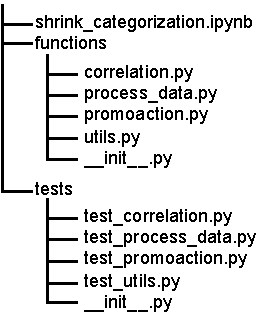
\includegraphics[width=.3\textwidth]{obrazky/strukturaslozky.pdf}
    \caption{Struktura souborů pro kód zpracovávající korelační analýzu.}
    \label{obr:strukturaslozky}
\end{figure}

Funkce jsou rozčleněny do modulů podle toho, na jaký výpočet jsou zaměřené. Každá funkce má je zdokumentovaná pomocí docstring obsaženého ve své definici. Dokumentace funkce se skládá ze stručného popisu, co funkce dělá, jaké má vstupní parametry a jaký je jejich význam a co funkce vrací. Funkce jsou otestované pomocí unit testů.

Pro práci s~tabulkovými daty, které jsou hlavním vstupem, jsem použila balíček \emph{pandas} jazyka Python. 
Pro otestování důležitých funkcí jsem použila knihovnu \emph{pytest}. 


% \emph{V~závorce je nástin toho, co budu popisovat (TBD)}

% \begin{itemize}
%     \item Výběr kategorie (Aby se nemuselo zadávat, přesné názvy kategorií systém vybere prvních $n$ nejsilnějších kategorií z~pohledu shrinků.)
%     \item Propojení dat
%     \item Korelace (Pearsonův, Spearmanův korelační koeficient) (ověření předpokladů (Kolmogorov-Smirnov test pro IID), testování statistické významnosti)
%     \item Kategorizace (Nastavení prahu pro velikost korelačního koeficientu)
%     \item Pomocné funkce
% \end{itemize}

\subsubsection*{Funkce pro přiřazení kategorií k~produktům}

Jak je uvedeno na začátku sekce \ref*{ss:vstupyvystupy}, uživatel musí specifikovat názvy sloupců kategorií, které bude v~analýze používat. Seznam těchto kategorií je pak parametrem pro funkci \texttt{assign\_levels}. Další parametry jsou DataFrame, kam se mají kategorie napojit a DataFrame odkud se kategorie napojují. Tyto DataFramy musí mít společný sloupec, podle kterého se napojení provede. Defaultně se jedná o sloupec s~ID produktu. Defaulně se provádí \emph{left join}, aby nedošlo ke ztrátě dat, kdyby nějaký produkt neměl v~DataFramu kategorií zastoupení. Funkci je také možné předat další argumenty, které se dají volat ve funkci \texttt{merge} knihovny \emph{pandas}. V~analýze shrinků jeden řádek dat odpovídá transakci jednoho produktu, proto byl zvoleno ID produktu jako propojovací sloupec.

\subsubsection*{Funkce pro vytipování rizikových kategorií}

Funkce \texttt{define\_risk\_categories} vybere prvních $n$ kategorií v~dané produktové hierarchii, kde suma hodnot v~dané kategorii, je nejvyšší, resp. nejnižší. Funkce vrací seznam těchto kategorií. Prvním vstupní parametrem je DataFrame, který obsahuje minimálně tři sloupce. Tyto sloupce je třeba definovat jako další parametry funkce. Jedná se o~sloupec \texttt{value\_column}, ve kterém jsou hodnoty, které ohodnocují řádky DataFramu a kategorie. Další sloupec je jedna z~úrovní produktové hierarchie, ve sloupci se nachází názvy, nebo jiné označení, kategorií. Posledním povinným parametrem je počet kategorií, které má funkce vrátit. Pokud je zadán tento počet tak, že je větší než je počet unikátních kategorií, vrátí se všechny kategorie seřazené od nejrizikovější. Dale je funkci možné předat keyword argumenty, které se předají funkci \texttt{sort\_values} z~knihovny \emph{pandas}. Jedná se např. o~parametr pro vzestupné, nebo sestupné řazení. Defaultní řazení je vzestupné, což znamená, že se vezmou kategorie s~nejnižší hodnotou. V~této analýze sledujeme vyhozené množství, resp. peníze. Tento ukazatel je záporný, tedy vzestupné řazení vybere ty kategorie, jejichž ztráta byla nejvyšší. Vrácený seznam kategorií je tedy seřazen od nejrizikovější kategorie.

\subsubsection*{Funkce pro výběr pouze dané kategorie ze všech záznamů}
Ve funkci \texttt{select\_category} jsou vstupem DataFrame, název kategorie a úroveň, ve které se daná kategorie nachází. Funkce vrací DataFrame pouze s~těmi řádky, kde je obsažena jmenovaná kategorie. V~případě, že tato kategorie v~datech není, je vrácen prázdný DataFrame.

Tato funkce je volána ve funkci \texttt{process\_dataframes}. Vstupy jsou totožné, avšak namísto jednoho DataFramu je možné jich zadat více jako samostatné parametry. 
% Tělo funkce je v~kódu \ref*{code:processdf}. 
Funkce vrací seznam všech vstupních DataFramů, a to pouze řádky, které obsahují zadanou kategorii.

% \begin{lstlisting}[language=Python,style=mystyle, label={code:processdf},  caption={Funkce pro výběr pouze dané katageorie z~více DataFramů.}]
% def process_dataframes(category: str, category_column: str, *dataframes) -> list[pd.DataFrame]:
%     result_dataframes = []

%     print("Sizes of dataframes: ")

%     for df in dataframes:
%         result_df = select_category(df, category, category_column)
%         print("Shape of original df: " , df.shape, "Shape of new df: " , result_df.shape)
%         result_dataframes.append(result_df)

%     return result_dataframes
% \end{lstlisting}

\subsubsection*{Funkce pro přiřazení promoakcí}

V rámci korelační analýzy bylo potřeba přiřadit k~jednotlivým zaznamenaným transakcím, zda byl produkt v~den záznamu v~promoakci nebo nikoli. V~ideálním případě by tento příznak mohl být již uvedený u každého záznamu. Pokud tomu tak, ale není, je nutné data o promocích provázat na základě data, produktu a prodejny podle číselníku promoakcí. Data vybrané společnosti, na jejíchž datech analýza probíhá, nemají promoakce přímo napojené na již proběhlé, zaznamenané transakce. Data o promoakcích jsou uložená v~číselníku promoakcí. Ten obsahuje ID produktu, prodejny, začátek a konec promoakce a prioritu promoakce. V~jeden den může být více promoakcí, v~takovém případě platí ta s~nejvyšší prioritou.

Základní funkce pro přiřazování promoakcí k~záznamům s~transakcemi se nazývá \texttt{map\_all\_promotions}. Tato funkce propojí DataFrame s~promoakcemi s~druhým DataFramem s~transakcemi. Může se jednat jak o záznamy shrinků, tak i o~prodeje. Důležité je, že tento DataFrame má sloupec s~datem, protože díky datu pak lze identifikovat správnou promoakci. Nalezení správné promoakce je implementováno až ve funkci \texttt{promo\_}, viz dále v~této sekci. Funkce \texttt{map\_all\_promotions} nejprve provede vnitřní spojení (neboli \emph{inner join}) obou vstupních DataFramů podle definovaných sloupců v~parametrech funkce. Tyto sloupce jsou vzhledem k~datům společnosti - sloupce s~ID produktu a ID prodejny. Tím je docíleno toho, že z~promoakcí získáme pouze ty záznamy pouze těch produktů, které se prodali, a které zároveň byly v~promoakci. Duplicitní záznamy se vynechají. U každého takového záznamu spočítá, kolikrát byl k~němu byla přiřazeno promoakce (tj.~kolik bylo promoakcí ve sledovaném období pro daný produkt a prodejnu) a ke~každému záznamu toto číslo přiřadí. Spolu s~číslem se přiřadí i identifikátor promoakce pro dvojici produkt-prodejna (viz tabulka C), tím je určena skupina k~sobě patřících záznamů. Takto označené záznamy se připojí k~původnímu DataFramu s~transakcemi. Záznamy, kde není žádná promoakce je počet promoakcí roven nule, zbylé hodnoty nejsou definované.
Dále se identifikátor upraví tak, že dokáže rozlišit unikátní promoakci na trojici produkt-prodejna-datum (viz tabulka D). V~tabulce \ref*{tab:tabulkypromoakceukaz} jsou umělá ukázková data, na kterých je znázorněno spojování dat.

\begin{table}[hbtp!]
    \centering
    \captionsetup{justification=centering}
    \caption{Umělá data pro znázornění přiřazování promoakcí k~transakcím.}
    \begin{tabular}{llll}
    \multicolumn{4}{c}{Tab. A: Tabulka promoakcí } \\
    \toprule
    ID produktu & Prodejna & Začátek promoakce & Konec promoakce  \\
    \midrule
    0001 & 01 & 2023-03-01 & 2023-03-05 \\
    0001 & 01 & 2023-03-15 & 2023-03-25 \\
    0002 & 02 & 2023-03-15 & 2023-03-25 \\
    0003 & 10 & 2023-03-15 & 2023-03-25 \\
    0004 & 02 & 2023-03-15 & 2023-03-25 \\
    \bottomrule
    \end{tabular}
\bigskip
    \begin{tabular}{lll}
        \multicolumn{3}{c}{Tab. B: Tabulka transakcí} \\
        \toprule
        Produkt & Prodejna & Datum transakce  \\
        \midrule
        0001 & 01 & 2023-03-02  \\
        0001 & 01 & 2023-03-09  \\
        0002 & 02 & 2023-03-15 \\
        0003 & 02 & 2023-03-15 \\
        0004 & 10 & 2023-03-15 \\
        0004 & 11 & 2023-03-30 \\
        \bottomrule
    \end{tabular}
\bigskip
    \begin{tabular}{llp{2cm}p{2.2cm}p{2cm}p{2cm}}
        \multicolumn{6}{c}{Tab. C: Tabulka souhlasných dvojic promoakce-produkt} \\
        \toprule
        Produkt & Prodejna & Začátek promoakce & Konec \newline promoakce& Identifikátor dvojice & Počet \newline  promoakcí\\
        \midrule
        0001 & 01 & 2023-03-01 & 2023-03-05 & 1 & 2\\
        0001 & 01 & 2023-03-15 & 2023-03-25 & 1 & 2\\
        0002 & 02 & 2023-03-15 & 2023-03-25 & 2 & 1\\
        \bottomrule
    \end{tabular}
\bigskip
    \begin{tabular}{llp{2cm}p{2cm}p{2.1cm}p{1.2cm}p{1.3cm}}
        \multicolumn{7}{c}{Tab. D: Tabulka souhlasných trojic promoakce-produkt-datum} \\
        \toprule
        Produkt & Prodejna & Datum transakce & Začátek promoakce & Konec \newline promoakce& Identi-\par fikátor trojice & Počet \newline promo-\par akcí\\
        \midrule
        0001 & 01 & 2023-03-02 & 2023-03-01 & 2023-03-05 & 1A & 2 \\
        0001 & 01 & 2023-03-02 & 2023-03-15 & 2023-03-25 & 1A & 2 \\
        0001 & 01 & 2023-03-09 & 2023-03-01 & 2023-03-05 & 1B & 2 \\
        0001 & 01 & 2023-03-09 & 2023-03-15 & 2023-03-25 & 1B & 2 \\
        0002 & 02 & 2023-03-15 & 2023-03-15 & 2023-03-25 & 2A & 1 \\
        0003 & 10 & 2023-03-15 & NaN & NaN & NaN & 0 \\
        0004 & 10 & 2023-03-15 & NaN & NaN & NaN & 0 \\
        0004 & 11 & 2023-03-30 & NaN& NaN & NaN & 0 \\
        \bottomrule
    \end{tabular}
    \label{tab:tabulkypromoakceukaz}
\end{table}

Z ukázky a z~popsaného postupu plyne, že výsledný DataFrame může mít více řádků než ten původní, ke kterému se přidávali promoakce. V~dalším kroku je tedy potřeba určit, která z~přiřazených promoakcí probíhala ve stejný čas jako je čas transakce. K~tomu jsem vytvořila funkci \texttt{label\_date\_with\_promo}. V~této funkci je každý řádek promoakce označen jednou ze tří možností: \texttt{no promo, promo, after promo}. Tedy zda je datum transakce během promoakce, nebo nikoli, nebo zda je v~rozmezí týden po evidované promoakci. Vzniklý příznak byl pojmenován jako typ promoakce. Ve~funkci se pracuje pouze se záznamy u nichž byla nalezena alespoň jedna možná promoakce, tj. transakce, kde dvojice produkt-prodejna existuje i v~promoakcích. Zbylé řádky tato funkce neoznačuje. V~tabulce \ref*{tab:tabulkalabely} jsou podle těchto pravidel označené jednotlivé řádky\footnote[1]{Zbylé sloupce jsou vynechané, protože pro ukázku příznaku nejsou podstatné.}.
 
\begin{table}[hbtp!]
    \centering
    \captionsetup{justification=centering}
    \caption{Tabulka transakcí a promoakcí s~přidaným příznakem typ promoakce.}
    \begin{tabular}{llp{2cm}p{2.1cm}p{2cm}p{2.5cm}}
        \toprule
        Produkt & Prodejna & Datum transakce & Začátek promoakce & Konec \newline promoakce& Typ \newline promoakce\\
        \midrule
        0001 & 01 & 2023-03-02 & 2023-03-01 & 2023-03-05 & promo \\
        0001 & 01 & 2023-03-02 & 2023-03-15 & 2023-03-25 & no promo \\
        0001 & 01 & 2023-03-09 & 2023-03-01 & 2023-03-05 & after promo \\
        0001 & 01 & 2023-03-09 & 2023-03-15 & 2023-03-25 & no promo \\
        0002 & 02 & 2023-03-15 & 2023-03-15 & 2023-03-25 & promo\\
        0003 & 10 & 2023-03-15 & NaN & NaN & no promo \\
        0004 & 10 & 2023-03-15 & NaN & NaN & no promo \\
        0004 & 11 & 2023-03-30 & NaN & NaN & no promo \\
        \bottomrule
    \end{tabular}
    \label{tab:tabulkalabely}
\end{table}

V dalším kroku je třeba vybrat pouze jednu přiřazenou promoakci o to se stará funkce \texttt{find\_duplicated\_records}. Tato funkce vrací seznam indexů řádků DataFramu, které se mohou zahodit. Algoritmus je znázorněný na obr. \ref*{label} \emph{TBD: obrázek UML}.
Postupně se prochází každý řádek DataFramu. v~pomocné proměnné se zaznamenává aktuální identifikátor určující jednoznačnou trojici produkt-prodejna-datum. Nejdříve se do pomocného seznamu nahrají všechny indexy řádků, které mají aktuální identifikátor. Potom se iteruje přes všechny tyto vybrané řádky. Pokud je typ promoakce iterovaného řádku typu \texttt{promo}, běh se zastaví a tento řádek se vybere ze skupiny záznamů, uloží se a pokračuje se na další skupinu. Pokud typ promoakce nebyl \texttt{promo}, ale \texttt{after promo}, tak se vybere tato promoakce, následné kroky jsou analogické předchozímu případu. Pokud nenastala ani jedna z~možností zbývá situace, kdy typ promoakce je \texttt{no promo}. Až jsou takto prohledané všechny záznamy, na základě seznamu vybraných řádkových indexů se vytvoří seznam indexů ke smazání jako rozdíl všech indexů v~DataFramu a indexů s~vybranými promoakcemi.

Funkce \texttt{match\_promo\_to\_sales} sdružuje dříve popsané funkce, které zpracovávají promoakce. Vstupními parametry funkce jsou DataFramy transakcí a promoakcí a názvy sloupců. Názvy sloupců mají předdefinovanou hodnotu, kterou lze změnit. v~dalším volitelném parametru je možné specifikovat formát datumu. Všechny slou-\\pce obsahující datumy se převedou na typ \texttt{datetime}. Poté se zavolá funkce \texttt{map\_all\_\\promotions}, která spojí transakce s~promoakcemi. Může vzniknout DataFrame, který má více řádků než původní. Výsledný DataFrame se předá funkci \texttt{label\_date\_\\with\_promo}, kde se označí u napojených promoakcích typ promoakce. Dále se pomocí funkce \texttt{find\_duplicated\_records} vyberou všechny řádky, které obsahují redundantní záznamy. Tyto řádky se odstraní z~DataFramu s~namapovanými promoakcemi. Ke všem řádkům, ke kterým neexistuje promoakce v~číselníku promoakcí, je přiřazen příznak \texttt{no promo}. Na závěr funkce zobrazí souhrn o velikostech dílčích DataFramů, aby měl uživatel informaci o počtech duplicitních záznamů. Během výpočtu jsou procesy iterování sledovány pomocí knihovny \emph{tqdm}.

\subsubsection*{Funkce pro korelační analýzu}

Funkce \texttt{aggregate\_sum} je pomocná funkce použitá v~kategorizaci produktů. Funkce agreguje vstupní DataFrame podle uvedených sloupců a sečte hodnoty ve všech numerických sloupcích. Ve~výsledném DataFramu resetuje označení řádků a vrátí ho.

Hodnoty korelačních koeficientů se počítají ve funkci \texttt{correlation}. Funkci je předán DataFrame a sloupce, kterých se korelace týká. Tato analýza je zaměřena na korelaci hodnoty shrinku s~dalšími ukazateli, proto je jedním vstupem název sloupce se shrinky a dalším vstupem je seznam sloupců ostatních ukazatelů. Obecně se nemusí jednat o~sloupec shrinků, základní myšlenkou ale je, že korelace je počítána pro každý sloupec ze seznam sloupců s~právě tímto jedním shrink sloupcem. Jedním z~volitelných parametrů funkce je určení metody pro získání korelačního koeficientu. Implementovány jsou dvě metody Pearsonův korelační koeficient a Spearmanův korelační koeficient. Pro výpočet jsou využité metody z~knihovny \emph{scipy}. Těmto metodám lze předat argument, zda se má uvažovat jednostranná nebo oboustranná alternativní hypotéza. Defaultní metodou je Pearsonův korelační koeficient a oboustranná alternativní hypotéza \cite{bib:scipyPearson}.

Před spuštěním výpočtů korelací jsou sloupce testované pro předpoklady IID. Pro testování, zda dva zkoumané sloupce patří do stejného rozdělení byl použitý Kolmo-\\gorov-Smirnovův test implementovaný v~knihovně \emph{scipy}. Pro nezávislost Ljung-Boxova metoda implementovaná v~knihovně \emph{statsmodels}.

Pro každý vypočtený koeficient je spočtena i $p$-hodnota, díky které lze hodnotu koeficientu označit za statisticky významnou, nebo ne. Pro určení významnosti byla implementována pomocná funkce \texttt{significance}. Ta vrací \texttt{True}, resp. \texttt{False} pro statisticky významné, resp. nevýznamné výsledky, tedy pokud je $p$-hodnota menší, resp. větší než $\alpha$. Předpokládaná hladina významnosti $\alpha$ je 5~\%. Výši hladiny lze změnit v~parametru funkce pro výpočet korelace, odtud se předá funkci pro určení významnosti. Vypočtené koeficienty a boolovský příznak o jejich významnosti se ukládají do dvou seznamů, které funkce vrací. Oba seznamy mají takový počet hodnot, jaká je délka vstupního seznamu sloupců.

V parametru \texttt{days} funkce \texttt{correlation} lze specifikovat, zda se má  korelace spočítat pouze mezi sloupcem shrinků se všemi sloupci ze seznamu sloupců anebo navíc se všemi sloupci ze seznami, kde jsou ale hodnoty v~tomto sloupci posunuté o parametr \texttt{days}. Pokud například \texttt{days=1}, pak k~hodnotě shrinku zaznamenané v~jistý den nebude náležet hodnota prodejů v~témže dni, ale hodnota ze dne předchozího. Tato volba byla přidána na základě hypotézy, že shrink se může projevit se zpožděním. Pokud jsou data takto posunutá, je třeba nahradit data na začátku sledovaného období. 
% v~současné implementaci jsou data nahrazená nulou, do budoucna by mohla být zvolena vhodná 

Funkce \texttt{product\_sales\_correlation} je zastřešující funkcí pro korelační analýzu na datových vstupech. Vstupními daty jsou DataFrame se záznamy shrinků a se záznamy prodejů včetně informace o promoakcích. K tomu je třeba definovat názvy  sloupců potřebných pro analýzu. Jedná se o sloupec s~hodnotami shrinků, hodnotou prodejů, ID produktů, ID prodejen a daty transakcí. Názvy sloupců mají defaultní hodnotu, kterou je samozřejmě možné změnit podle zkoumaných dat. Dále má funkce volitelný parametr \texttt{after\_promo}, jehož defaultní hodnota je \texttt{False}, který zohledňuje, zda se pro analýzu s~promočními prodeji použijí jen prodeje uskutečněné přímo během promoakce nebo i prodeje, které nastaly týden po promoakci. Další parametry jsou volitelné parametry, které se předávají funkcím, které jsou volány v~rámci zastřešující funkce (metoda, alternativní hypotéza, hladina významnosti, počet dní posunu). 

Funkce vrací tři proměnné. První je DataFrame, který obsahuje seznam produktů a ke každému z~nich napočítané korelační koeficienty hodnoty shrinku s~ukazateli a statistickou významnost tohoto koeficientu. Déle je vrácen seznam produktů, které neměly žádný promoční prodej ve sledovaném období a případně i produktů, které neměly žádný prodej.

Funkce nejprve vytiskne hlášku, která metoda pro výpočet korelace se použije. Poté se inicializují názvy sloupců pro ukládání korelací a příznaku o statistické významnosti. Počet sloupců se liší v~závislosti na tom, zda se v~analýze zkoumá i varianta se zpožděním shrinku oproti prodejům. Sloupce jsou seřazené tak, aby sloupce týkající se korelace s~jedním ukazatelem byly vedle sebe v~následujícím pořadí: korelační koeficient, statistická významnost, korelační koeficient se zpožděním, statistická významnost pro koeficient se zpožděním. Takto budou hodnoty uložené ve výsledném DataFramu. Pro všechny ukazatele se čtveřice (v případě zpoždění) nebo dvojice (bez zpoždění), opakuje. Dále se inicializuje prázdný DataFrame pro ukládání výsledků s~názvem sloupce pro ID produktu spolu s~nově vytvořenými názvy. 

Dále je třeba ze vstupního DataFramu prodejů vybrat pouze záznamy produktů, které se prodaly během promoakce. Pokud je parametr \texttt{after\_promo} je \texttt{True}, pak se kromě záznamů produktů v~promoakci vyberou i ty, kde produkty byly prodány v~rámci týdne po promoakci. Dále se inicializují prázdné seznamy pro uchování produktů, které nemají žádné prodeje, resp. promoční prodeje.

Následně probíhá iterace přes všechny unikátní produkty, pro které byl zaznamenaný shrink. Počet zkoumaných produktů se vytiskne. Na začátku každé iterace je třeba z~DataFramů shrinků vybrat pouze záznamy s~daným produktem. DataFrame se potom agreguje podle sloupců datum transakce a ID prodejny. Stejný postup se aplikuje pro DataFrame s~prodeji. Navíc se obdobný postup aplikuje i na DataFramy s~promočními záznamy a se všemi prodeji s~tím rozdílem, že se vyhledají záznamy všech produktů kromě iterovaného produktu. Výsledné DataFramy se potom sloučí do jednoho podle sloupců ID prodejny a datumu. Jelikož může nastat situace, že ne všechny hodnoty jsou definované na každém řádku, nahradí se nedefinované hodnoty nulou.

Na složený DataFrame se použije funkce \texttt{correlation}, které se předají příslušné parametry. Výsledky se pak vloží jako nový řádek do DataFramu pro ukládání výsledků. Pokud nebylo možné spočíst korelace, z~důvodu, že rozptyl hodnot byl nulový - nastane pokud produkt nemá žádné prodeje -  nahradíme nedefinovanou korelaci nulou, která indikuje, že mezi veličinami není závislost.

Výsledný DataFrame s~korelací je vstupem do funkce \texttt{categorization}.  Dalšími vstupy je název sloupce, který obsahuje korelačními koeficienty shrinků produktu s~jeho vlastními tržbami a sloupce s~koeficienty shrinků produktu s~prodeji ostatních produktů. Ve funkci se vytvoří nový DataFrame pro uložení výsledků kategorizace. Jeho indexem jsou ID produktů. Samotná kategorizace se získá spuštěním funkce \texttt{categorize\_products}, která vrací seznam kategorií pro každý řádek vstupního DataFramu. Funkce \texttt{categorize\_products} roztřídí produkty do pěti kategorií: \texttt{P, O, V, N, X}. Postup roztřídění produktů do těchto kategorií je popsaný v~sekci \ref{sec:kor:postup}.

Poté, co má každý produkt přiřazenou kategorii se ve funkci \texttt{categorization} označí každý produkt s~kategorií, zda je výsledek statisticky reprezentativní, nebo ne. Rozhodující hodnota je získána pomocí funkce \texttt{unsignificant\_rows}. Která vrací logickou hodnotu výroku:
$$ \mbox{Významnost}(r_i) \lor ( (\mbox{Koeficient(korelace produktu se sebou)} \leq 0) $$ 
$$ \land  \mbox{Významnost(korelace produktu s~ostatními)} ) $$
Funkce pak vrátí DataFrame s~takto označenými a kategorizovanými produkty.
% \texttt{categorization}, \texttt{categorize\_products}, \texttt{unsignificant\_rows}.

\subsubsection*{Pomocné funkce}

Funkce \texttt{create\_folder} vytvoří složku se zadaným jménem v~aktuální cestě, pouze pokud již taková složka neexistuje. Další pomocná funkce je \texttt{format\_date}, která využívá funkci z~knihovny \emph{pandas} \texttt{to\_datetime}. 
Pro základní vizualizaci korelace mezi sloupci jsem vytvořila funkci, která pomocí knihovny \emph{matplotlib} vytváří bodový graf dvou proměnných. Graf je buď uložen nebo zobrazený při spuštění funkce. Funkci lze předat DataFrame a názvy dvou sloupců, které reprezentují vstupy pro osy $x$ a $y$ grafu. Další vstupy jsou názvy os a grafu, případně název souboru, pokud uživatel graf uložit.

Pro vizualizaci výsledků byla implementována funkce \texttt{create\_waffle\_chart}, pomocí knihovny \emph{plotly}. Tato knihovna umožňuje vytvářet interaktivní grafy pro pro-\\ středí Jupyter Notebook. Výsledky jsou zobrazené pomocí tzv. vaflového grafu. Jednotlivé produkty jsou zobrazeny jako buňky v~mřížce. Jsou barevně odlišené podle   typu kategorie, do které byl produkt klasifikován. Výhodou tohoto typu grafu je, že na první pohled lze vidět relativní četnost jednotlivých kategorií. Při najetí na pole mřížky se zobrazí tooltip (při zobrazení grafu v~Jupyter Notebooku, ve kterém je vytvoření grafu spouštěno) s informacemi o produktu. Vedle grafu je zobrazena legenda, která kromě názvu příslušné kategorie zobrazuje kolik procent tato kategorie v~ dané skupině produkt tvoří. Ukázka se nachází v~ sekci s~výsledky na obr. \ref*{obr:kor:vyslMASO}.

% \textbf{Testování}

% Pro testování důležitých funkcí jsem použila knihovnu \emph{pytest} jazyka Python. 
% Testy lze spustit příkazem \texttt{python -m pytest tests} v~kořenovém adresáři projektu.


\section{Výsledky}

Analýza se týká pouze dat jednoho měsíce a kategorií produktů první úrovně \emph{Velmi čerstvé}, zastoupena 48~\% a \emph{Čerstvé}, zastoupena 52~\% ve vybraných datech. Data obsahují pouze jeden typ shrinku -- prošlé a zkažené zboží, který zaujímá téměř 65~\% shrinků pro dané kategorie. Zastoupení typů shrinků, které zabírají v~datech více jak dvě procenta se nachází v~tabulce \ref*{tab:shrinkyZastoupeni}.
Zaměřila jsem se na kategorie ze čtvrté úrovně, a to prvních deset kategorií s~nejvyšší hodnotou shrinků (tj. s~nejvyšší zaznamenanou ztrátou). V~práci jsou popsány výsledky pouze tří kategorií -- Masné výrobky -- pultový prodej, Slané pečivo a Plodová zelenina. Na třetím místě byla kategorie Sladké pečivo, ale kvůli podobnosti s~druhou kategorií, jsem zvolila následující kategorii v~pořadí vzhledem k~hodnotě shrinku.
V~tabulce \ref*{tab:lostcost4} jsou procentuální hodnoty zastoupení čtyř kategorií mezi ostatními kategoriemi úrovně 4 podle velikosti shrinku. 

\begin{table}[h!]
    \begin{center}
            \captionsetup{justification=centering}
    \caption{Zastoupení vybraných shrinků ve zkoumaných datech \\(kategorie Čerstvé a Velmi čerstvé).}
    \begin{tabular}{l r}
        Typ shrinku & Zastoupení v~kategoriích [\%]\\
        \midrule
        Prošlé a zkažené zboží & $64{,}97$ \\
        Potravinová banka & $23{,}72$ \\
        Poškození & $6{,}26$ \\
        Zvířecí útulky & $2{,}69$ \\
        Kompostéry &  $2{,}36$ \\
        \end{tabular}
    \label{tab:shrinkyZastoupeni}
\end{center}
\end{table}

\begin{table}[h!]
    \centering
    \captionsetup{justification=centering}
    \caption{Tabulka čtyř kategorií ze čtvrté úrovně produktové hierarchie podle zastoupení zaznamenané hodnoty shrinku na všech evidovaných shrincích.}
    \begin{tabular}{l r}
        Kategorie & Zastoupení [\%] \\

    \hline
    Masné výrobky -- pultový prodej &$ 26{,}27$ \\
    Slané pečivo&  $12{,}12$\\
    Sladké pečivo&   $6{,}82$\\
    Plodová zelenina&   $5{,}65$\\
    \end{tabular}
    \label{tab:lostcost4}
    \end{table}

Měřila jsem postupně korelaci velikosti shrinku s~různými ukazateli pro celkové tržby ostatních produktů. Pro určení míry korelace jsem zvolila Spearmanův korelační koeficient, jelikož data nesplňují předpoklady, které jsou nutné pro použití Pearsonova korelačního koeficientu - data nejsou nezávislá a stejně rozdělená. Data vybrané společnosti, také nesplňují podmínku normality. To může být dáno tím, že data pochází z~reálného světa a zaznamenávají jev, který závisí na mnoha, těžce predikovatelných faktorech. Nejprve jsem zvolila 5\% hladinu významnosti pro testování statistické významnosti koeficientů korelace $r_\mathrm{P}$ a $r_\mathrm{O}$. Výsledky ovšem ukázaly, že alespoň hodnoty třetiny produktů ve zkoumaných kategoriích  byly neprůkazné. Rozhodla jsem se tedy zvýšit hladinu významnosti na 10~\%. Zvýšení hladiny významnosti zvýšilo pravděpodobnost vzniku chyby druhého druhu, nicméně případné zařazení produktu do špatné kategorie nemá z~businessového hlediska fatální následky.

Na obrázcích~\ref*{obr:kategCorrPorovnani} až~\ref*{obr:kategCorrPorovnaniZel} jsou porovnání výsledků kategorizace pro zmíněné tři kategorie. Pokaždé bylo spuštěno šest výpočtů. Korelace byla měřena mezi shrinky a tržbami ostatních produktů, ostatních produktů, kde prodeje byly posunuté o jeden den, dále mezi shrinky a tržbami produktů v~promoakci a produktů v~promoakci s~posunem prodejů. Varianty s~promoakcemi dále byly jak pro shrinky produktů během promoakce, tak pro během i po promoakci. Na obrázcích jsou zobrazené výsledky pro variantu během i po promoakci, protože zachytila stejně nebo více případů než varianta záznamů pouze během promoakce. 

Z~uvedených počtů produktů u jednotlivých kategoriích pro různé ukazatele, je patrné, že výsledky se příliš neliší. Pokud bychom se ale zaměřovali na celkové prodeje, nikoli promoční, tak získáváme větší množství produktů, u~nichž nebylo možné vysvětlit shrink pomocí korelace. Avšak hypotézy pro rozřazení produktů uvažují právě promoční prodeje nikoli celkové prodeje. Další popis se věnuje výsledkům korelace mezi shrinky a promočními a popromočními prodeji, které měly stejný den záznamu jako shrink, na obrázcích ~\ref*{obr:kategCorrPorovnani} až~\ref*{obr:kategCorrPorovnaniZel} se jedná o poslední řádek s~výsledky.
% Nejvíce zařazených produktů bylo pro kategorie 

\begin{figure}[h!]
    \centering
    \captionsetup{justification=centering}
    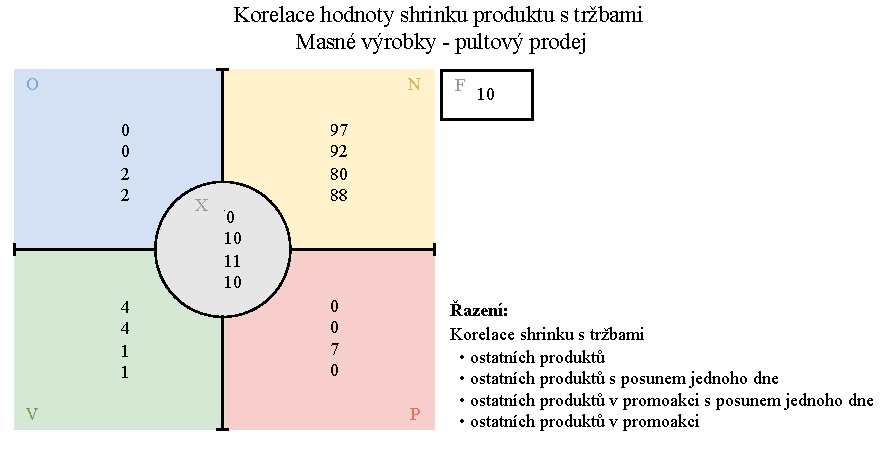
\includegraphics[width=\textwidth]{obrazky/kor_maso.pdf}
    \caption{Počet produktů z~kategorie Masné výrobky -- pultový prodej roztříděné pomocí korelační analýzy v~závislosti na různých ukazatelích.}
    \label{obr:kategCorrPorovnani}
\end{figure}

\begin{figure}[h!]
    \centering
    \captionsetup{justification=centering}
    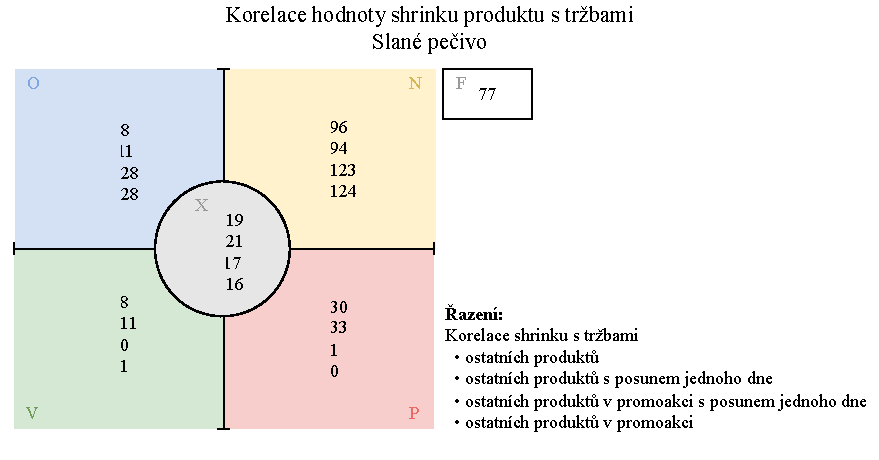
\includegraphics[width=\textwidth]{obrazky/kor_pec.pdf}
    \caption{Počet produktů z~kategorie Slané pečivo roztříděné pomocí korelační analýzy v~závislosti na různých ukazatelích.}
    \label{obr:kategCorrPorovnaniPec}
\end{figure}

\begin{figure}[h!]
    \centering
    \captionsetup{justification=centering}
    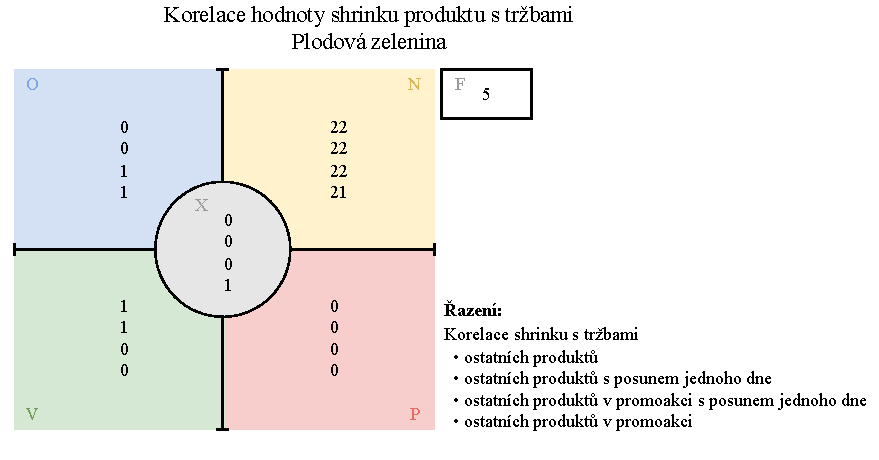
\includegraphics[width=\textwidth]{obrazky/kor_zel.pdf}
    \caption{Počet produktů z~kategorie Plodová zelenina roztříděné pomocí korelační analýzy v~závislosti na různých ukazatelích.}
    \label{obr:kategCorrPorovnaniZel}
\end{figure}

% \begin{table}[hbtp!]
%     \centering
%     \captionsetup{justification=centering}
%     \caption{Počet produktů v~kategoriích v~závislosti na různých ukazatelích. Kategorizace proběhla na základě Spearmanova korelačního koeficientu}
%     \begin{tabular}{l *{6}{r}}
%     \toprule
%     \multicolumn{1}{l}{} & \multicolumn{6}{c}{Korelace s~tržbami ostatních produktů} \\
%     \multicolumn{1}{l}{} & \multicolumn{2}{c}{Všechny prodeje} & \multicolumn{2}{c}{Prodeje v~promoakci}  & \multicolumn{2}{c}{Prodeje v~a po promoakci} \\
%     Kategorie & Stejný den & Další den & Stejný den & Další den & Stejný den & Další den \\
%     \midrule
%     \multicolumn{7}{c}{Masné výrobky -- pultový prodej} \\
%     \midrule
%     P           & 96   & 96   & 96   & 96   & 96   & 96   \\
%     O           & 1     & 1   & 2   & 2   & 2   & 2   \\
%     X           & 3     & 3   & 2   & 2   & 2   & 2   \\
%     Nevýzn.     & 11    & 11   & 11   & 11   & 11   & 11   \\
%     \midrule
%     \multicolumn{7}{c}{Slané pečivo} \\
%     \midrule
%     P           & 131   & 131   & 131   & 131   & 131   & 131   \\
%     O           & 9     & 13   & 24   & 24   & 24   & 24   \\
%     X           & 16    & 12   & 1    & 1    & 1    & 1    \\
%     Nevýzn.     & 90    & 90   & 90   & 90   & 90   & 90   \\
%     \bottomrule
%     \end{tabular}
%     \label{tab:kategCorrPorovnani}
% \end{table}

\textbf{Masné výrobky -- pultový prodej}

Shrink byl zaznamenaný u 111 produktů v~této kategorii úrovně 4. 88 produktů bylo klasifikováno jako kategorie N, deset jako kategorie X, dva jako kategorie O, jeden jako V. U zbylých deseti produktů nebyl koeficient korelace statisticky významný, a proto nejde u těchto produktů vyslovit hypotézu pro jejich zařazení. Korelace mezi hodnotou shrinku a promočními tržbami je na obr. \ref*{obr:corr:maso}.

\begin{figure}[h!]
    \centering
    \captionsetup{justification=centering}
    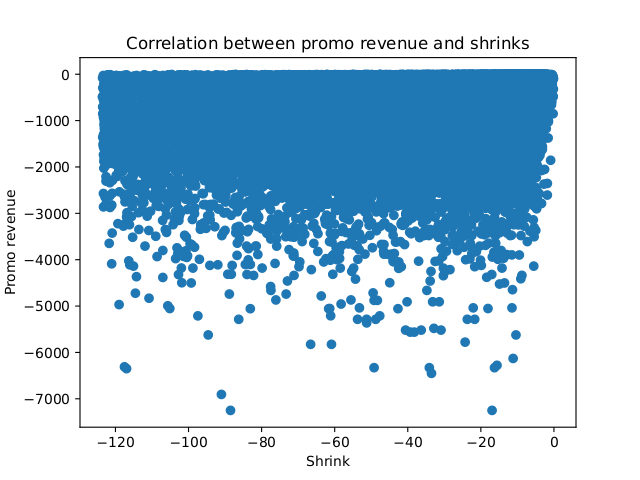
\includegraphics[width=.8\textwidth]{obrazky/grafy/categorization_charts/categorization_charts_L4_PROCMEAT.png}
    \caption{Závislost mezi tržbami produktu a tržbami ostatních produktů \\ v~kategorii během promoakce (Masné výrobky -- pultový prodej).}
    \label{obr:corr:maso}
\end{figure}

Produkty, které patří do kategorie O: Velikonoční klobása a Velikonoční šunka - jedná se zcela jistě o sezónní výrobky. Produkt, který byl označen jako výprodejový jsou Párky (Kuřecí striptýzky). Šest produktů z~kategorie nemělo během sledovaného období žádné evidované prodeje, všechny byly klasifikovány jako kategorie X, tedy hodnota koeficientu korelace neznamenala závislost. %{TODO: vyjmenovat i další produkty, které si způsobují samy, ale je to většina produktů a salámy, šunky, z~kategorie...} 

Dále jsem zkoumala podkategorie Masných výrobků. Porovnávala jsem prodeje v~rámci kategorií na šesté úrovni produktové hierarchie. V~podkategorii Salámy s~krátkou dobou spotřeby se kategorizace potvrdila. Pro kategorii, do níž patří sezónní výrobky - Netučné masné výrobky, nově z~této podkategorie byl jako kategorie O označen i produkt Kladenská pečeně.

Na obr. \ref*{obr:kor:vyslMASO} se nachází vizualizace získaných výsledků vygenerovaný pomocí Python knihovny \emph{plotly}. Při najetí na příslušné políčko (v~Jupyter Notebooku) se zobrazí údaje o produktu.

\begin{figure}[h!]
    \centering
    \captionsetup{justification=centering}
    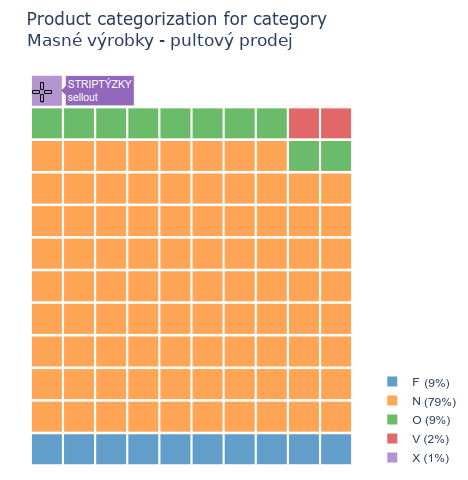
\includegraphics[width=.7\textwidth]{obrazky/zntb/vysledekMASO.png}
    \caption{Vizualizace výsledků rozdělení přiřazených kategorií \\ pro kategorii produktů Masné výrobky -- pultový prodej.}
    \label{obr:kor:vyslMASO}
\end{figure}


\textbf{Slané pečivo}

Shrink byl zaznamenaný u 246 produktů. 124 produktů bylo klasifikováno jako kategorie N, 16 jako kategorie X, 28 jako kategorie O, jeden jako P. Pro 77 produktů nebyl koeficient korelace statisticky významný. Jako produkt, který si způsobuje shrinky sám, byl označený obyčejný rohlík. Rohlík se tedy vyhazuje více čím vyšší jsou jeho vlastní tržby. Celkově patří tento produkt mezi ty s~největšími shrinky.

Produkty, které byly zařazeny do kategorie X, tj. takové, u kterých nebyl koeficient korelace dostatečně velký, byly produkty, které neměly během sledovaného období žádný prodej (promoční, či nepromoční).

% Produkty, které patří do kategorie O:
% pletýnka adélka, pletýnka malena, pletýnka sypaná mákem, pletýnka sypaná solí a km., bramborové pečivo s~cibulí, veka cupeko kb, rohlík grahamový aspec, rohlík pivní ora, rohlík staročeský, rohlík obilný mam, rohlík na strouh.karlova, rohl.n str.penam, houska mašek, houska raženka, bageta rust.poh., bageta s~grahamem, bageta chlebová, banketka cereální, dalamánek, kostka cereál malena, ciabatta mini natural, twistr se sýrem a špenatem, anglický rohlík, 

% \textbf{Sladké pečivo}

% % čokorolka, závin mák , skořicový vrut, donut bílý se sušnkami, závitek cereální nugátový, rohlík lístový s~ořech. náp, kobliha vanilková šiška, kobliha vanilková v~koš, kobliha s~jablky a skořicí, kobliha s~lísko.náp.a pol, koblih kapsa s~jablky, koláč wellartův, koláč tlač. vícezrnný, koláč šátek makový, koláč s~ovocnou nápl, koláček švestkový , koláček meruňkový , koláček borůvkový, koláč rohový tři náplně , koláč s~makovou náplní, koláč s~tvarohovo nápl, máslový koláč tvaroh, šátek kyn. tvarohová nápl, šáteček s~náplní višňovou , šáteček s~tvaroh.náplní, šátek makový, loupák o., loupák v., loupák m., závin tvaroh , závin kvásk. makový, bavorská hvězdice, makovka pletená mašek, croissant máslový

\textbf{Plodová zelenina}

Shrink byl zaznamenaný u 28 produktů v~této kategorii. 21 produktů bylo klasifikováno jako kategorie N, jeden produkt jako X a jeden jako O. U ostatních pěti produktů nebyl koeficient dostatečně významný. Produkt, který v~této kategorii neměl žádné prodeje byl pouze Lilek Bio, pro který koeficient korelace byl označen jako nevýznamný. Produkt, z~kategorie O, byla Cherry rajčata. Zatímco produkt z~ktegorie X, byl Paprika barevná Mix.

% product_id	warehouse_id	date_of_transaction	amount	cost_value	motive_type	weekday	quarter	warehouse_type	region	...	amount_share	whs_cost_value_share	promotion_type_1_id	promo	L1	L3	L4	L1_cost_value_share	L5	L6
% 0	24293174	644	2023-03-01	-0.47	-52.29	4	2	1	SM	Praha	...	0.1423	0.000005	NaN	no promo	SUPERFRESH	SF CM RED MEAT	RED MEAT	0.000060	MIX OF RED MEAT CHILLED	READY TO COOK RED MEAT CHILLED
% 1	26973548	644	2023-03-01	-2.00	-49.00	4	2	1	SM	Praha	...	0.0667	0.000005	NaN	no promo	SUPERFRESH	SF CM PROCESSED F&V	FRESH PROCESSED FV	0.000056	FRESH PROCESSED VEGETABLES	FRESH PROCESSED VEGETABLES SNACK
% 2	20428587	644	2023-03-01	-27.00	-44.55	4	2	1	SM	Praha	...	0.0076	0.000004	NaN	no promo	SUPERFRESH	SF CM BAKERY	SALTY PASTRY	0.000051	FRESH PASTRY BASIC	BUNS & KAISERKA
% 3	20480905	644	2023-03-01	-66.00	-106.26	4	2	1	SM	Praha	...	0.0082	0.000010	NaN	no promo	SUPERFRESH	SF CM BAKERY	SALTY PASTRY	0.000121	FRESH PASTRY BASIC	ROLL BASIC
% 4	23309074	644	2023-03-01	-1.00	-43.17	4	2	1	SM	Praha	...	0.1429	0.000004	NaN	no promo	SUPERFRESH	SF CM BAKERY	FRESH CONFECTIONARY	0.000049	FRESH CONFECTIONARY DESSERTS	FRESH DESSERTS
% 5 rows × 24 columns

% (811526, 24)
% product_id	promotion_type_1_id	promotion_date_from	promotion_date_to	warehouse_id	L3	L4	L5	L6	name
% 0	27630563	1	2023-02-22	2023-03-07	526	NaN	NaN	NaN	NaN	NaN
% 1	27653944	1	2023-02-22	2023-03-07	526	SF CM RED MEAT	RED MEAT	BEEF MEAT CHILLED	READY TO COOK RED MEAT CHILLED	BIO MASOVÉ KULIČKY 300G
% 2	27669921	1	2023-02-22	2023-03-07	526	FF CM CONVENIENCE	CHILLED PRODUCT SELF SERVICE	FRESH DELI PESTO & SAUCES SELF SERVICE	FRESH DELI VEGETARIAN SAUCES	NP VE BIO ORIENTAL TASTE 300G
% 3	27692653	1	2023-02-22	2023-03-07	526	FF CM CONVENIENCE	CHILLED PRODUCT SELF SERVICE	FRESH DELI PICKLED PRODUCTS SELF SERVICE	FRESH DELI PICKLED VEGETABLE	NP VE BIO KIMCHI NEPÁLIVÉ 350G
% 4	21817410	1	2023-02-22	2023-03-07	526	SF CM RED MEAT	RED MEAT	BEEF MEAT CHILLED	JOINT BEEF CHILLED	NP BIO HOV.ZADNÍ BK NA PEČENÍ
% (5539222, 10)
% product_id	warehouse_id	date_of_transaction	amount	cost_value	promotion_id	position_type	document_type_id	L3	L4	L5	L6	name	warehouse_type
% 0	20008963	820	2023-03-23	-1.0	-88.00	\N	2	150	NaN	NaN	NaN	NaN	NaN	HM
% 1	20013059	152	2023-03-14	-1.0	-25.38	\N	0	150	NaN	NaN	NaN	NaN	NaN	HM
% 2	20013059	152	2023-03-17	-4.0	-101.52	\N	0	150	NaN	NaN	NaN	NaN	NaN	HM
% 3	20013059	152	2023-03-19	-1.0	-25.38	\N	0	150	NaN	NaN	NaN	NaN	NaN	HM
% 4	20013059	152	2023-03-23	-1.0	-25.38	\N	0	150	NaN	NaN	NaN	NaN	NaN	HM
% (36575915, 14)

% ====================================================================================================================================================
% ====================================================================================================================================================
% ====================================================================================================================================================
% ====================================================================================================================================================
% MEAT
% % \begin{itemize}
% %     \itemsep0em 

% %     \item oboustranná: korelace je nenulová,
% %     \item jednostranná (menší než nula): korelace je záporná
% %     \item jednostranná (větší než nula): korelace je kladná
% % \end{itemize}

% %  MEAT PRODUCTS
% % Catgeorization:  correlation_with_other_products:
% % itself    96
% % False     11
% % None       3
% % other      1
% % Catgeorization:  correlation_with_other_products_past:
% % itself    96
% % False     11
% % None       4
% % Catgeorization:  correlation_with_other_products_promo:
% % itself    96
% % False     11
% % other      2
% % None       2
% % Catgeorization:  correlation_with_other_products_promo_past:
% % itself    96
% % False     11
% % other      2
% None       2

% Analyzing category: SALTY PASTRY of L4 category level.
% ======================================================
% Sizes of dataframes with obly the selected category: 
% Shape of df:  (104427, 22)
% Shape of df:  (8944, 10)
% Shape of df:  (480412, 14)
% Labeling promotions.
% 234020it [01:02, 3733.68it/s]
% Searching for duplicate records.
% 234020it [00:36, 6353.39it/s] 
% Count of rows to drop:  104772
% Shapes of dataframes: Sales:  (477631, 14) Promotions:  (8944, 10) Sales with promo:  (582403, 19) Sales with promo no duplicates:  (477631, 17)
% Calculating  spearman  correlation coefficient.
% Number of products in category:  246

% Products that had no sales during promotion:  223 products.
% Products that had no sales at all:  18 products.
% [22459466, 23194175, 26109718, 27344064, 22095022, 26627342, 21488931, 21976056, 21976124, 22045751, 26627328, 26778808, 25773071, 27735190, 27684436, 27740767, 27710340, 27740750]
% Catgeorization:  correlation_with_other_products:
% itself    131
% False      90
% None       16
% other       9

% Catgeorization:  correlation_with_other_products_past:
% itself    131
% False      90
% None       14
% other      11

% Catgeorization:  correlation_with_other_products_promo:
% itself    131
% False      90
% other      24
% None        1

% Catgeorization:  correlation_with_other_products_promo_past:
% itself    131
% False      90
% other      24
% None        1

% Analyzing category: FRUIT VEGETABLE of L4 category level.
% =========================================================
% Sizes of dataframes with obly the selected category: 
% Shape of df:  (34680, 22)
% Shape of df:  (5556, 10)
% Shape of df:  (179351, 14)
% Labeling promotions.
% 114262it [00:30, 3747.84it/s]
% Searching for duplicate records.
% 114262it [00:13, 8487.78it/s] 
% Count of rows to drop:  49439
% Shapes of dataframes: Sales:  (177703, 14) Promotions:  (5556, 10) Sales with promo:  (227142, 19) Sales with promo no duplicates:  (177703, 17)
% Calculating  spearman  correlation coefficient.
% Number of products in category:  28

% Products that had no sales during promotion:  16 products.
% [20444853, 20445836, 20698171, 26398969, 24363303, 20452094, 20445553, 21497513, 20446086, 27299395, 24228862, 24391078, 26977775, 23930742, 27227947, 27333501]
% Products that had no sales at all:  1 products.
% [27333501]
% Catgeorization:  correlation_with_other_products:
% itself    20
% False      8

% Catgeorization:  correlation_with_other_products_past:
% itself    20
% False      8

% Catgeorization:  correlation_with_other_products_promo:
% itself    20
% False      8

% Catgeorization:  correlation_with_other_products_promo_past:
% itself    20
% False      8

% Analyzing category: SWEET PASTRY of L4 category level.
% ======================================================
% Sizes of dataframes with obly the selected category: 
% Shape of df:  (48701, 22)
% Shape of df:  (16131, 10)
% Shape of df:  (634294, 14)
% Labeling promotions.
% 304122it [01:18, 3892.35it/s]
% Searching for duplicate records.
% 304122it [00:41, 7351.05it/s]
% Count of rows to drop:  24675
% Shapes of dataframes: Sales:  (632724, 14) Promotions:  (16131, 10) Sales with promo:  (657399, 19) Sales with promo no duplicates:  (632724, 17)
% Calculating  spearman  correlation coefficient.
% Number of products in category:  386

% Products that had no sales during promotion:  331 products.
% Products that had no sales at all:  10 products.
% [22055101, 27729915, 26159140, 26778860, 21976186, 26778846, 27738740, 27737170, 21976209, 27636015]
% Catgeorization:  correlation_with_other_products:
% False     197
% itself    155
% None       34

% Catgeorization:  correlation_with_other_products_past:
% False     197
% itself    155
% None       30
% other       4

% Catgeorization:  correlation_with_other_products_promo:
% False     197
% itself    155
% other      34

% Catgeorization:  correlation_with_other_products_promo_past:
% False     197
% itself    155
% other      34

% Analyzing category: RED MEAT of L4 category level.
% ==================================================
% Sizes of dataframes with obly the selected category: 
% Shape of df:  (17391, 22)
% Shape of df:  (29066, 10)
% Shape of df:  (332815, 14)
% Labeling promotions.
% 390190it [01:35, 4092.89it/s]
% Searching for duplicate records.
% 390190it [00:50, 7735.99it/s] 
% Count of rows to drop:  174298

% Products that had no sales during promotion:  65 products.
% [24293174, 24560115, 25720938, 24125499, 27725788, 24646864, 26040561, 26042824, 22840400, 26044910, 26566849, 26123615, 26130309, 26045061, 26045016, 27669778, 26045030, 26159881, 27166031, 22840387, 25881493, 26123677, 22257628, 26045115, 26124872, 26915975, 25960051, 26044811, 27712375, 25615036, 26872667, 26277202, 26770987, 26725192, 26044927, 26277226, 26177038, 27712399, 26044989, 27557235, 26770901, 27522660, 26643885, 26771007, 26771120, 27133279, 26157870, 26125275, 27743164, 26835846, 26871677, 26157733, 27102176, 26954905, 27260081, 27098868, 27103715, 27260265, 27738474, 27100912, 27425893, 27738481, 26566856, 27743157, 26771137]
% Products that had no sales at all:  17 products.
% [27725788, 26123615, 26130309, 26159881, 27166031, 26123677, 26124872, 26044989, 27133279, 26125275, 27743164, 26157733, 27098868, 27103715, 27738474, 27738481, 27743157]
% Catgeorization:  correlation_with_other_products:
% itself    96
% False     39
% None       3


% Catgeorization:  correlation_with_other_products_past:
% itself    96
% False     39
% None       3


% Catgeorization:  correlation_with_other_products_promo:
% itself    96
% False     39
% other      3


% Catgeorization:  correlation_with_other_products_promo_past:
% itself    96
% False     39
% other      3

% % https://docs.scipy.org/doc/scipy/reference/generated/scipy.stats.spearmanr.html
% % https://statistics.laerd.com/statistical-guides/spearmans-rank-order-correlation-statistical-guide-2.php There is no [monotonic] association between the two variables [in the population].






% Analyzing category: PROC. MEAT SERVICE of L4 category level.
% ============================================================
% Sizes of dataframes with obly the selected category: 
% Shape of df:  (303847, 22)
% Shape of df:  (70584, 10)
% Shape of df:  (555853, 14)
% Labeling promotions.
% 1679273it [08:33, 3270.31it/s]
% Searching for duplicate records.
% 1679273it [04:13, 6615.74it/s]
% Count of rows to drop:  1165224
% Shapes of dataframes: Sales:  (554305, 14) Promotions:  (70584, 10) Sales with promo:  (1719529, 19) Sales with promo no duplicates:  (554305, 17)
% Method:  pearson  after promo:  False
% Calculating  pearson  correlation coefficient.
% Number of products in category:  111

% Products that had no sales during promotion:  40 products.
% [20454081, 20454111, 25666854, 25961225, 26872896, 23180666, 20453978, 23373204, 24888967, 25478198, 25726787, 25961164, 26831718, 26831817, 27254783, 27571781, 27627761, 25726299, 25961140, 27150054, 25726046, 25726015, 25842371, 27571774, 20402082, 26835587, 25959000, 27722930, 27571798, 27736982, 27254486, 25726060, 27739174, 27737033, 27738504, 26835624, 27738733, 27611357, 25842579, 26831824]
% Products that had no sales at all:  6 products.
% [27722930, 27736982, 27739174, 27737033, 27738504, 27738733]
% Method:  pearson  after promo:  False
% Catgeorization:  correlation_with_other_products:
% itself    100
% False       9
% None        2


% Catgeorization:  correlation_with_other_products_past:
% itself    100
% False       9
% None        2


% Catgeorization:  correlation_with_other_products_promo:
% itself    100
% False       9
% other       1
% None        1


% Catgeorization:  correlation_with_other_products_promo_past:
% itself    100
% False       9
% other       1
% None        1


% Method:  spearman  after promo:  False
% Calculating  spearman  correlation coefficient.
% Number of products in category:  111
% Products that had no sales during promotion:  40 products.
% [20454081, 20454111, 25666854, 25961225, 26872896, 23180666, 20453978, 23373204, 24888967, 25478198, 25726787, 25961164, 26831718, 26831817, 27254783, 27571781, 27627761, 25726299, 25961140, 27150054, 25726046, 25726015, 25842371, 27571774, 20402082, 26835587, 25959000, 27722930, 27571798, 27736982, 27254486, 25726060, 27739174, 27737033, 27738504, 26835624, 27738733, 27611357, 25842579, 26831824]
% Products that had no sales at all:  6 products.
% [27722930, 27736982, 27739174, 27737033, 27738504, 27738733]
% Method:  spearman  after promo:  False
% Catgeorization:  correlation_with_other_products:
% itself    96
% False     11
% None       3
% other      1


% Catgeorization:  correlation_with_other_products_past:
% itself    96
% False     11
% None       3
% other      1


% Catgeorization:  correlation_with_other_products_promo:
% itself    96
% False     11
% other      2
% None       2


% Catgeorization:  correlation_with_other_products_promo_past:
% itself    96
% False     11
% other      2
% None       2


% Method:  pearson  after promo:  True
% Calculating  pearson  correlation coefficient.
% Number of products in category:  111
% Products that had no sales during promotion:  32 products.
% [26872896, 24888967, 25478198, 25726787, 25961164, 26831718, 26831817, 27254783, 27571781, 27627761, 25726299, 25961140, 27150054, 25726046, 25726015, 27571774, 20402082, 26835587, 25959000, 27722930, 27571798, 27736982, 27254486, 25726060, 27739174, 27737033, 27738504, 26835624, 27738733, 27611357, 25842579, 26831824]
% Products that had no sales at all:  6 products.
% [27722930, 27736982, 27739174, 27737033, 27738504, 27738733]
% Method:  pearson  after promo:  True
% Catgeorization:  correlation_with_other_products:
% itself    100
% False       9
% None        2


% Catgeorization:  correlation_with_other_products_past:
% itself    100
% False       9
% None        2


% Catgeorization:  correlation_with_other_products_promo:
% itself    100
% False       9
% other       1
% None        1


% Catgeorization:  correlation_with_other_products_promo_past:
% itself    100
% False       9
% other       1
% None        1


% Method:  spearman  after promo:  True
% Calculating  spearman  correlation coefficient.
% Number of products in category:  111
% Products that had no sales during promotion:  32 products.
% [26872896, 24888967, 25478198, 25726787, 25961164, 26831718, 26831817, 27254783, 27571781, 27627761, 25726299, 25961140, 27150054, 25726046, 25726015, 27571774, 20402082, 26835587, 25959000, 27722930, 27571798, 27736982, 27254486, 25726060, 27739174, 27737033, 27738504, 26835624, 27738733, 27611357, 25842579, 26831824]
% Products that had no sales at all:  6 products.
% [27722930, 27736982, 27739174, 27737033, 27738504, 27738733]
% Method:  spearman  after promo:  True
% Catgeorization:  correlation_with_other_products:
% itself    96
% False     11
% None       4


% Catgeorization:  correlation_with_other_products_past:
% itself    96
% False     11
% None       4


% Catgeorization:  correlation_with_other_products_promo:
% itself    96
% False     11
% other      2
% None       2


% Catgeorization:  correlation_with_other_products_promo_past:
% itself    96
% False     11
% other      2
% None       2


% Analyzing category: SALTY PASTRY of L4 category level.
% ======================================================
% Sizes of dataframes with obly the selected category: 
% Shape of df:  (104427, 22)
% Shape of df:  (8944, 10)
% Shape of df:  (480412, 14)
% Labeling promotions.
% 234020it [01:11, 3260.33it/s]
% Searching for duplicate records.
% 234020it [00:30, 7668.35it/s] 
% Count of rows to drop:  104772
% Shapes of dataframes: Sales:  (477631, 14) Promotions:  (8944, 10) Sales with promo:  (582403, 19) Sales with promo no duplicates:  (477631, 17)
% Method:  pearson  after promo:  False
% Calculating  pearson  correlation coefficient.
% Number of products in category:  246
% Products that had no sales during promotion:  227 products.
% [20428587, 20480905, 21852039, 23472266, 25467697, 27422731, 27442449, 27456934, 27516850, 27516867, 27544884, 27544907, 27544952, 27544983, 27578025, 27609699, 25672985, 26782034, 27544914, 27544938, 23472259, 27123195, 27544877, 27544891, 27603581, 25310863, 26576442, 26627373, 27123201, 27274750, 27574270, 22459466, 23194175, 23549074, 25895667, 26109718, 26737430, 26737461, 26737478, 27266038, 27269244, 27344064, 27603598, 27619810, 22095022, 26627342, 27638019, 20783808, 21488931, 21976056, 21976124, 22045751, 26627328, 26709468, 27442760, 27312759, 26737539, 26778808, 21471971, 24587136, 27544969, 25318074, 25322194, 25892369, 26960975, 25512700, 23319905, 25673005, 23635739, 25516234, 26359205, 25012200, 25175639, 25431483, 25430783, 25430837, 25430820, 25773071, 27075234, 27075227, 25629620, 26571362, 26571324, 26571331, 27601532, 26786698, 27710418, 22941404, 25504422, 27034071, 26975085, 27449943, 25548761, 25663075, 27195000, 24744881, 27641569, 26445540, 27201930, 22957733, 27374993, 22962294, 25426496, 25426502, 25254792, 27610640, 25506242, 26546117, 27610664, 27735190, 25507294, 25507256, 25506297, 25506303, 22993847, 22993885, 25504439, 25504460, 25571608, 25431599, 27329290, 21482922, 24174381, 25390261, 25390254, 25390643, 25394368, 24328579, 25665864, 24644167, 27329269, 25594836, 22933904, 22933973, 27619513, 27384039, 27384053, 25393422, 25891966, 27134641, 27134634, 23549067, 27152706, 25665802, 25605327, 26787008, 25630602, 26035062, 27455630, 25504446, 27620175, 25571615, 25571660, 27134658, 27134665, 27134689, 24323611, 25498554, 25630596, 25630619, 27619520, 26802046, 27134719, 26975740, 27603611, 25513318, 27282670, 27696729, 27466261, 22993892, 22662200, 25630466, 22019943, 27712306, 27684436, 27278116, 26381350, 26885506, 27307656, 26389400, 27329139, 22516657, 27329184, 27329115, 27032404, 27215937, 26386973, 27453179, 27715444, 25756999, 27128473, 26347394, 27136768, 25661224, 24277365, 25048698, 26434582, 27152492, 27715451, 23478992, 26975078, 26391175, 26802060, 25326185, 26381459, 26576848, 24644143, 25605273, 25066159, 25630657, 26581798, 27574225, 26975689, 27620182, 26381381, 24704427, 26975764, 24644150, 22126221, 25504491, 27710432, 27740767, 27710340, 26502755, 27312827, 27740750, 26579221]
% Products that had no sales at all:  18 products.
% [22459466, 23194175, 26109718, 27344064, 22095022, 26627342, 21488931, 21976056, 21976124, 22045751, 26627328, 26778808, 25773071, 27735190, 27684436, 27740767, 27710340, 27740750]
% Method:  pearson  after promo:  False
% Catgeorization:  correlation_with_other_products:
% itself    130
% False     100
% None       13
% other       3


% Catgeorization:  correlation_with_other_products_past:
% itself    130
% False     100
% None       11
% other       5


% Catgeorization:  correlation_with_other_products_promo:
% itself    130
% False     100
% other      16


% Catgeorization:  correlation_with_other_products_promo_past:
% itself    130
% False     100
% other      16


% Method:  spearman  after promo:  False
% Calculating  spearman  correlation coefficient.
% Number of products in category:  246
% Products that had no sales during promotion:  227 products.
% [20428587, 20480905, 21852039, 23472266, 25467697, 27422731, 27442449, 27456934, 27516850, 27516867, 27544884, 27544907, 27544952, 27544983, 27578025, 27609699, 25672985, 26782034, 27544914, 27544938, 23472259, 27123195, 27544877, 27544891, 27603581, 25310863, 26576442, 26627373, 27123201, 27274750, 27574270, 22459466, 23194175, 23549074, 25895667, 26109718, 26737430, 26737461, 26737478, 27266038, 27269244, 27344064, 27603598, 27619810, 22095022, 26627342, 27638019, 20783808, 21488931, 21976056, 21976124, 22045751, 26627328, 26709468, 27442760, 27312759, 26737539, 26778808, 21471971, 24587136, 27544969, 25318074, 25322194, 25892369, 26960975, 25512700, 23319905, 25673005, 23635739, 25516234, 26359205, 25012200, 25175639, 25431483, 25430783, 25430837, 25430820, 25773071, 27075234, 27075227, 25629620, 26571362, 26571324, 26571331, 27601532, 26786698, 27710418, 22941404, 25504422, 27034071, 26975085, 27449943, 25548761, 25663075, 27195000, 24744881, 27641569, 26445540, 27201930, 22957733, 27374993, 22962294, 25426496, 25426502, 25254792, 27610640, 25506242, 26546117, 27610664, 27735190, 25507294, 25507256, 25506297, 25506303, 22993847, 22993885, 25504439, 25504460, 25571608, 25431599, 27329290, 21482922, 24174381, 25390261, 25390254, 25390643, 25394368, 24328579, 25665864, 24644167, 27329269, 25594836, 22933904, 22933973, 27619513, 27384039, 27384053, 25393422, 25891966, 27134641, 27134634, 23549067, 27152706, 25665802, 25605327, 26787008, 25630602, 26035062, 27455630, 25504446, 27620175, 25571615, 25571660, 27134658, 27134665, 27134689, 24323611, 25498554, 25630596, 25630619, 27619520, 26802046, 27134719, 26975740, 27603611, 25513318, 27282670, 27696729, 27466261, 22993892, 22662200, 25630466, 22019943, 27712306, 27684436, 27278116, 26381350, 26885506, 27307656, 26389400, 27329139, 22516657, 27329184, 27329115, 27032404, 27215937, 26386973, 27453179, 27715444, 25756999, 27128473, 26347394, 27136768, 25661224, 24277365, 25048698, 26434582, 27152492, 27715451, 23478992, 26975078, 26391175, 26802060, 25326185, 26381459, 26576848, 24644143, 25605273, 25066159, 25630657, 26581798, 27574225, 26975689, 27620182, 26381381, 24704427, 26975764, 24644150, 22126221, 25504491, 27710432, 27740767, 27710340, 26502755, 27312827, 27740750, 26579221]
% Products that had no sales at all:  18 products.
% [22459466, 23194175, 26109718, 27344064, 22095022, 26627342, 21488931, 21976056, 21976124, 22045751, 26627328, 26778808, 25773071, 27735190, 27684436, 27740767, 27710340, 27740750]
% Method:  spearman  after promo:  False
% Catgeorization:  correlation_with_other_products:
% itself    131
% False      90
% None       16
% other       9


% Catgeorization:  correlation_with_other_products_past:
% itself    131
% False      90
% other      13
% None       12


% Catgeorization:  correlation_with_other_products_promo:
% itself    131
% False      90
% other      24
% None        1


% Catgeorization:  correlation_with_other_products_promo_past:
% itself    131
% False      90
% other      24
% None        1


% Method:  pearson  after promo:  True
% Calculating  pearson  correlation coefficient.
% Number of products in category:  246
% 246it [01:23,  2.93it/s]
% Products that had no sales during promotion:  223 products.
% [20428587, 20480905, 21852039, 23472266, 25467697, 27442449, 27456934, 27516850, 27516867, 27544884, 27544907, 27544952, 27544983, 27578025, 27609699, 25672985, 26782034, 27544914, 27544938, 23472259, 27123195, 27544877, 27544891, 25310863, 26576442, 26627373, 27123201, 27274750, 27574270, 22459466, 23194175, 23549074, 25895667, 26109718, 26737430, 26737461, 26737478, 27266038, 27269244, 27344064, 27619810, 22095022, 26627342, 27638019, 20783808, 21488931, 21976056, 21976124, 22045751, 26627328, 26709468, 27442760, 27312759, 26737539, 26778808, 21471971, 24587136, 27544969, 25318074, 25322194, 25892369, 25512700, 23319905, 25673005, 23635739, 25516234, 26359205, 25012200, 25175639, 25431483, 25430783, 25430837, 25430820, 25773071, 27075234, 27075227, 25629620, 26571362, 26571324, 26571331, 27601532, 26786698, 27710418, 22941404, 25504422, 27034071, 26975085, 27449943, 25548761, 25663075, 27195000, 24744881, 27641569, 26445540, 27201930, 22957733, 27374993, 22962294, 25426496, 25426502, 25254792, 27610640, 25506242, 26546117, 27610664, 27735190, 25507294, 25507256, 25506297, 25506303, 22993847, 22993885, 25504439, 25504460, 25571608, 25431599, 27329290, 21482922, 24174381, 25390261, 25390254, 25390643, 25394368, 24328579, 25665864, 24644167, 27329269, 25594836, 22933904, 22933973, 27619513, 27384039, 27384053, 25393422, 25891966, 27134641, 27134634, 23549067, 27152706, 25665802, 25605327, 26787008, 25630602, 26035062, 27455630, 25504446, 27620175, 25571615, 25571660, 27134658, 27134665, 27134689, 24323611, 25498554, 25630596, 25630619, 27619520, 26802046, 27134719, 26975740, 27603611, 25513318, 27282670, 27696729, 27466261, 22993892, 22662200, 25630466, 22019943, 27712306, 27684436, 27278116, 26381350, 26885506, 27307656, 26389400, 27329139, 22516657, 27329184, 27329115, 27032404, 27215937, 26386973, 27453179, 27715444, 25756999, 27128473, 26347394, 27136768, 25661224, 24277365, 25048698, 26434582, 27152492, 27715451, 23478992, 26975078, 26391175, 26802060, 25326185, 26381459, 26576848, 24644143, 25605273, 25066159, 25630657, 26581798, 27574225, 26975689, 27620182, 26381381, 24704427, 26975764, 24644150, 22126221, 25504491, 27710432, 27740767, 27710340, 26502755, 27312827, 27740750, 26579221]
% Products that had no sales at all:  18 products.
% [22459466, 23194175, 26109718, 27344064, 22095022, 26627342, 21488931, 21976056, 21976124, 22045751, 26627328, 26778808, 25773071, 27735190, 27684436, 27740767, 27710340, 27740750]
% Method:  pearson  after promo:  True
% Catgeorization:  correlation_with_other_products:
% itself    130
% False     100
% None       14
% other       2


% Catgeorization:  correlation_with_other_products_past:
% itself    130
% False     100
% None       13
% other       3


% Catgeorization:  correlation_with_other_products_promo:
% itself    130
% False     100
% other      16


% Catgeorization:  correlation_with_other_products_promo_past:
% itself    130
% False     100
% other      16


% Method:  spearman  after promo:  True
% Products that had no sales during promotion:  223 products.
% [20428587, 20480905, 21852039, 23472266, 25467697, 27442449, 27456934, 27516850, 27516867, 27544884, 27544907, 27544952, 27544983, 27578025, 27609699, 25672985, 26782034, 27544914, 27544938, 23472259, 27123195, 27544877, 27544891, 25310863, 26576442, 26627373, 27123201, 27274750, 27574270, 22459466, 23194175, 23549074, 25895667, 26109718, 26737430, 26737461, 26737478, 27266038, 27269244, 27344064, 27619810, 22095022, 26627342, 27638019, 20783808, 21488931, 21976056, 21976124, 22045751, 26627328, 26709468, 27442760, 27312759, 26737539, 26778808, 21471971, 24587136, 27544969, 25318074, 25322194, 25892369, 25512700, 23319905, 25673005, 23635739, 25516234, 26359205, 25012200, 25175639, 25431483, 25430783, 25430837, 25430820, 25773071, 27075234, 27075227, 25629620, 26571362, 26571324, 26571331, 27601532, 26786698, 27710418, 22941404, 25504422, 27034071, 26975085, 27449943, 25548761, 25663075, 27195000, 24744881, 27641569, 26445540, 27201930, 22957733, 27374993, 22962294, 25426496, 25426502, 25254792, 27610640, 25506242, 26546117, 27610664, 27735190, 25507294, 25507256, 25506297, 25506303, 22993847, 22993885, 25504439, 25504460, 25571608, 25431599, 27329290, 21482922, 24174381, 25390261, 25390254, 25390643, 25394368, 24328579, 25665864, 24644167, 27329269, 25594836, 22933904, 22933973, 27619513, 27384039, 27384053, 25393422, 25891966, 27134641, 27134634, 23549067, 27152706, 25665802, 25605327, 26787008, 25630602, 26035062, 27455630, 25504446, 27620175, 25571615, 25571660, 27134658, 27134665, 27134689, 24323611, 25498554, 25630596, 25630619, 27619520, 26802046, 27134719, 26975740, 27603611, 25513318, 27282670, 27696729, 27466261, 22993892, 22662200, 25630466, 22019943, 27712306, 27684436, 27278116, 26381350, 26885506, 27307656, 26389400, 27329139, 22516657, 27329184, 27329115, 27032404, 27215937, 26386973, 27453179, 27715444, 25756999, 27128473, 26347394, 27136768, 25661224, 24277365, 25048698, 26434582, 27152492, 27715451, 23478992, 26975078, 26391175, 26802060, 25326185, 26381459, 26576848, 24644143, 25605273, 25066159, 25630657, 26581798, 27574225, 26975689, 27620182, 26381381, 24704427, 26975764, 24644150, 22126221, 25504491, 27710432, 27740767, 27710340, 26502755, 27312827, 27740750, 26579221]
% Products that had no sales at all:  18 products.
% [22459466, 23194175, 26109718, 27344064, 22095022, 26627342, 21488931, 21976056, 21976124, 22045751, 26627328, 26778808, 25773071, 27735190, 27684436, 27740767, 27710340, 27740750]
% Method:  spearman  after promo:  True
% Catgeorization:  correlation_with_other_products:
% itself    131
% False      90
% None       16
% other       9


% Catgeorization:  correlation_with_other_products_past:
% itself    131
% False      90
% None       14
% other      11


% Catgeorization:  correlation_with_other_products_promo:
% itself    131
% False      90
% other      24
% None        1


% Catgeorization:  correlation_with_other_products_promo_past:
% itself    131
% False      90
% other      24
% None        1


% ./categorization_charts/categorization_charts_L4_SALTY PASTRY.pdf
% Analyzing category: FRUIT VEGETABLE of L4 category level.
% =========================================================
% Sizes of dataframes with obly the selected category: 
% Shape of df:  (34680, 22)
% Shape of df:  (5556, 10)
% Shape of df:  (179351, 14)
% Labeling promotions.
% 114262it [00:29, 3873.93it/s]
% Searching for duplicate records.
% 114262it [00:14, 8118.47it/s]
% Count of rows to drop:  49439
% Shapes of dataframes: Sales:  (177703, 14) Promotions:  (5556, 10) Sales with promo:  (227142, 19) Sales with promo no duplicates:  (177703, 17)
% Method:  pearson  after promo:  False
% Calculating  pearson  correlation coefficient.
% Number of products in category:  28

% Products that had no sales during promotion:  17 products.
% [20444853, 20445836, 20698171, 26398969, 24363303, 20452094, 20445553, 21497513, 20446086, 27299395, 24228862, 24391078, 27186244, 26977775, 23930742, 27227947, 27333501]
% Products that had no sales at all:  1 products.
% [27333501]
% Method:  pearson  after promo:  False
% Catgeorization:  correlation_with_other_products:
% itself    23
% False      5


% Catgeorization:  correlation_with_other_products_past:
% itself    23
% False      5


% Catgeorization:  correlation_with_other_products_promo:
% itself    23
% False      5


% Catgeorization:  correlation_with_other_products_promo_past:
% itself    23
% False      5


% Method:  spearman  after promo:  False
% Calculating  spearman  correlation coefficient.
% Number of products in category:  28

% Products that had no sales during promotion:  17 products.
% [20444853, 20445836, 20698171, 26398969, 24363303, 20452094, 20445553, 21497513, 20446086, 27299395, 24228862, 24391078, 27186244, 26977775, 23930742, 27227947, 27333501]
% Products that had no sales at all:  1 products.
% [27333501]
% Method:  spearman  after promo:  False
% Catgeorization:  correlation_with_other_products:
% itself    20
% False      8


% Catgeorization:  correlation_with_other_products_past:
% itself    20
% False      8


% Catgeorization:  correlation_with_other_products_promo:
% itself    20
% False      8


% Catgeorization:  correlation_with_other_products_promo_past:
% itself    20
% False      8


% Method:  pearson  after promo:  True
% Calculating  pearson  correlation coefficient.
% Number of products in category:  28

% Products that had no sales during promotion:  16 products.
% [20444853, 20445836, 20698171, 26398969, 24363303, 20452094, 20445553, 21497513, 20446086, 27299395, 24228862, 24391078, 26977775, 23930742, 27227947, 27333501]
% Products that had no sales at all:  1 products.
% [27333501]
% Method:  pearson  after promo:  True
% Catgeorization:  correlation_with_other_products:
% itself    23
% False      5


% Catgeorization:  correlation_with_other_products_past:
% itself    23
% False      5


% Catgeorization:  correlation_with_other_products_promo:
% itself    23
% False      5


% Catgeorization:  correlation_with_other_products_promo_past:
% itself    23
% False      5


% Method:  spearman  after promo:  True
% Calculating  spearman  correlation coefficient.
% Number of products in category:  28

% Products that had no sales during promotion:  16 products.
% [20444853, 20445836, 20698171, 26398969, 24363303, 20452094, 20445553, 21497513, 20446086, 27299395, 24228862, 24391078, 26977775, 23930742, 27227947, 27333501]
% Products that had no sales at all:  1 products.
% [27333501]
% Method:  spearman  after promo:  True
% Catgeorization:  correlation_with_other_products:
% itself    20
% False      8


% Catgeorization:  correlation_with_other_products_past:
% itself    20
% False      8


% Catgeorization:  correlation_with_other_products_promo:
% itself    20
% False      8


% Catgeorization:  correlation_with_other_products_promo_past:
% itself    20
% False      8


% ./categorization_charts/categorization_charts_L4_FRUIT VEGETABLE.pdf
% Analyzing category: SWEET PASTRY of L4 category level.
% ======================================================
% Sizes of dataframes with obly the selected category: 
% Shape of df:  (48701, 22)
% Shape of df:  (16131, 10)
% Shape of df:  (634294, 14)
% Labeling promotions.
% 304122it [01:10, 4326.14it/s]
% Searching for duplicate records.
% 304122it [00:43, 6952.49it/s]
% Count of rows to drop:  24675
% Shapes of dataframes: Sales:  (632724, 14) Promotions:  (16131, 10) Sales with promo:  (657399, 19) Sales with promo no duplicates:  (632724, 17)
% Method:  pearson  after promo:  False
% Calculating  pearson  correlation coefficient.
% Number of products in category:  386

% Products that had no sales during promotion:  339 products.

% Products that had no sales at all:  10 products.
% [22055101, 27729915, 26159140, 26778860, 21976186, 26778846, 27738740, 27737170, 21976209, 27636015]
% Method:  pearson  after promo:  False
% Catgeorization:  correlation_with_other_products:
% False     228
% itself    143
% None       15


% Catgeorization:  correlation_with_other_products_past:
% False     228
% itself    143
% None       15


% Catgeorization:  correlation_with_other_products_promo:
% False     228
% itself    143
% other      15


% Catgeorization:  correlation_with_other_products_promo_past:
% False     228
% itself    143
% other      15


% Method:  spearman  after promo:  False
% Calculating  spearman  correlation coefficient.
% Number of products in category:  386

% Products that had no sales at all:  10 products.
% [22055101, 27729915, 26159140, 26778860, 21976186, 26778846, 27738740, 27737170, 21976209, 27636015]
% Method:  spearman  after promo:  False
% Catgeorization:  correlation_with_other_products:
% False     197
% itself    155
% None       34


% Catgeorization:  correlation_with_other_products_past:
% False     197
% itself    155
% None       31
% other       3


% Catgeorization:  correlation_with_other_products_promo:
% False     197
% itself    155
% other      34


% Catgeorization:  correlation_with_other_products_promo_past:
% False     197
% itself    155
% other      34


% Method:  pearson  after promo:  True
% Calculating  pearson  correlation coefficient.
% Number of products in category:  386

% Products that had no sales at all:  10 products.
% [22055101, 27729915, 26159140, 26778860, 21976186, 26778846, 27738740, 27737170, 21976209, 27636015]
% Method:  pearson  after promo:  True
% Catgeorization:  correlation_with_other_products:
% False     228
% itself    143
% None       15


% Catgeorization:  correlation_with_other_products_past:
% False     228
% itself    143
% None       15


% Catgeorization:  correlation_with_other_products_promo:
% False     228
% itself    143
% other      15


% Catgeorization:  correlation_with_other_products_promo_past:
% False     228
% itself    143
% other      15


% Method:  spearman  after promo:  True
% Calculating  spearman  correlation coefficient.
% Number of products in category:  386
% Method:  spearman  after promo:  True
% Catgeorization:  correlation_with_other_products:
% False     197
% itself    155
% None       34


% Catgeorization:  correlation_with_other_products_past:
% False     197
% itself    155
% None       30
% other       4


% Catgeorization:  correlation_with_other_products_promo:
% False     197
% itself    155
% other      34


% Catgeorization:  correlation_with_other_products_promo_past:
% False     197
% itself    155
% other      34


% ./categorization_charts/categorization_charts_L4_SWEET PASTRY.pdf
% Analyzing category: RED MEAT of L4 category level.
% ==================================================
% Sizes of dataframes with obly the selected category: 
% Shape of df:  (17391, 22)
% Shape of df:  (29066, 10)
% Shape of df:  (332815, 14)
% Labeling promotions.
% 390190it [01:53, 3428.34it/s]
% Searching for duplicate records.
% 390190it [00:53, 7325.67it/s] 
% Count of rows to drop:  174298
% Shapes of dataframes: Sales:  (331211, 14) Promotions:  (29066, 10) Sales with promo:  (505509, 19) Sales with promo no duplicates:  (331211, 17)
% Method:  pearson  after promo:  False
% Calculating  pearson  correlation coefficient.
% Number of products in category:  138
% Products that had no sales at all:  17 products.
% [27725788, 26123615, 26130309, 26159881, 27166031, 26123677, 26124872, 26044989, 27133279, 26125275, 27743164, 26157733, 27098868, 27103715, 27738474, 27738481, 27743157]
% Method:  pearson  after promo:  False
% Catgeorization:  correlation_with_other_products:
% itself    98
% False     36
% None       4


% Catgeorization:  correlation_with_other_products_past:
% itself    98
% False     36
% None       4


% Catgeorization:  correlation_with_other_products_promo:
% itself    98
% False     36
% other      3
% None       1


% Catgeorization:  correlation_with_other_products_promo_past:
% itself    98
% False     36
% other      3
% None       1


% Method:  spearman  after promo:  False
% Calculating  spearman  correlation coefficient.
% Number of products in category:  138
% Method:  spearman  after promo:  False
% Catgeorization:  correlation_with_other_products:
% itself    96
% False     39
% None       3


% Catgeorization:  correlation_with_other_products_past:
% itself    96
% False     39
% None       3


% Catgeorization:  correlation_with_other_products_promo:
% itself    96
% False     39
% other      3


% Catgeorization:  correlation_with_other_products_promo_past:
% itself    96
% False     39
% other      3


% Method:  pearson  after promo:  True
% Calculating  pearson  correlation coefficient.
% Number of products in category:  138
% Catgeorization:  correlation_with_other_products:
% itself    98
% False     36
% None       4


% Catgeorization:  correlation_with_other_products_past:
% itself    98
% False     36
% None       4


% Catgeorization:  correlation_with_other_products_promo:
% itself    98
% False     36
% other      3
% None       1


% Catgeorization:  correlation_with_other_products_promo_past:
% itself    98
% False     36
% other      3
% None       1


% Method:  spearman  after promo:  True
% Calculating  spearman  correlation coefficient.
% Number of products in category:  138
% Method:  spearman  after promo:  True
% Catgeorization:  correlation_with_other_products:
% itself    96
% False     39
% None       3


% Catgeorization:  correlation_with_other_products_past:
% itself    96
% False     39
% None       3


% Catgeorization:  correlation_with_other_products_promo:
% itself    96
% False     39
% other      3


% Catgeorization:  correlation_with_other_products_promo_past:
% itself    96
% False     39
% other      3


% ./categorization_charts/categorization_charts_L4_RED MEAT.pdf
% Analyzing category: BREAD of L4 category level.
% ===============================================
% Sizes of dataframes with obly the selected category: 
% Shape of df:  (28750, 22)
% Shape of df:  (3463, 10)
% Shape of df:  (394320, 14)
% Labeling promotions.
% 90421it [00:27, 3314.86it/s]
% Searching for duplicate records.
% 90421it [00:15, 5783.06it/s]
% Count of rows to drop:  43979
% Products that had no sales at all:  86 products.
% [27062715, 26778785, 27711200, 27529997, 27722800, 27710319, 25586015, 25597301, 25586855, 25586657, 25586688, 27131466, 27259528, 25586053, 25586725, 25589535, 27727461, 25586695, 25589627, 25589832, 25586848, 27247105, 27247129, 25586763, 25586114, 25586107, 25586701, 25586664, 25586862, 25586879, 25586060, 25586596, 25586909, 25586916, 25586602, 25586619, 25665147, 25586138, 25586503, 25586091, 25586084, 25586077, 25586411, 25586404, 27643822, 26804934, 27710333, 27643839, 25585988, 25586787, 26804903, 26316208, 25589924, 25589542, 25586893, 25589528, 25715651, 25589856, 27625378, 27711286, 26316451, 27711293, 25589580, 27745670, 25589825, 25589870, 27750216, 27745663, 25586046, 25665130, 27746509, 27754238, 25586022, 26410692, 27735039, 25586718, 25586794, 25586121, 27750193, 25586039, 25589672, 25586671, 25589818, 25586770, 27758731, 27747117]
% Method:  pearson  after promo:  False
% Catgeorization:  correlation_with_other_products:
% False     255
% itself    143
% None       21


% Catgeorization:  correlation_with_other_products_past:
% False     255
% itself    143
% None       20
% other       1


% Catgeorization:  correlation_with_other_products_promo:
% False     255
% itself    143
% other      13
% None        8


% Catgeorization:  correlation_with_other_products_promo_past:
% False     255
% itself    143
% other      13
% None        8


% Method:  spearman  after promo:  False
% Calculating  spearman  correlation coefficient.
% Number of products in category:  419
% Method:  spearman  after promo:  False
% Catgeorization:  correlation_with_other_products:
% False     225
% itself    157
% None       29
% other       8


% Catgeorization:  correlation_with_other_products_past:
% False     225
% itself    157
% None       26
% other      11


% Catgeorization:  correlation_with_other_products_promo:
% False     225
% itself    157
% other      24
% None       13


% Catgeorization:  correlation_with_other_products_promo_past:
% False     225
% itself    157
% other      23
% None       14


% Method:  pearson  after promo:  True
% Calculating  pearson  correlation coefficient.
% Number of products in category:  419
% Method:  pearson  after promo:  True
% Catgeorization:  correlation_with_other_products:
% False     255
% itself    143
% None       21


% Catgeorization:  correlation_with_other_products_past:
% False     255
% itself    143
% None       21


% Catgeorization:  correlation_with_other_products_promo:
% False     255
% itself    143
% other      13
% None        8


% Catgeorization:  correlation_with_other_products_promo_past:
% False     255
% itself    143
% other      13
% None        8


% Method:  spearman  after promo:  True
% Calculating  spearman  correlation coefficient.
% Number of products in category:  419
% Method:  spearman  after promo:  True
% Catgeorization:  correlation_with_other_products:
% False     225
% itself    157
% None       27
% other      10


% Catgeorization:  correlation_with_other_products_past:
% False     225
% itself    157
% None       26
% other      11


% Catgeorization:  correlation_with_other_products_promo:
% False     225
% itself    157
% other      24
% None       13


% Catgeorization:  correlation_with_other_products_promo_past:
% False     225
% itself    157
% other      23
% None       14


% ./categorization_charts/categorization_charts_L4_BREAD.pdf
% Analyzing category: CITRUSES of L4 category level.
% ==================================================
% Sizes of dataframes with obly the selected category: 
% Shape of df:  (26646, 22)
% Shape of df:  (6364, 10)
% Shape of df:  (88119, 14)
% Labeling promotions.
% 153368it [00:41, 3657.83it/s]
% Searching for duplicate records.
% 153368it [00:20, 7608.09it/s]
% Count of rows to drop:  79062
% Shapes of dataframes: Sales:  (86946, 14) Promotions:  (6364, 10) Sales with promo:  (166008, 19) Sales with promo no duplicates:  (86946, 17)
% Method:  pearson  after promo:  False
% Calculating  pearson  correlation coefficient.
% Number of products in category:  15
% Products that had no sales during promotion:  5 products.
% [25225501, 20441012, 25405729, 20442071, 27755990]
% Products that had no sales at all:  1 products.
% [27755990]
% Method:  pearson  after promo:  False
% Catgeorization:  correlation_with_other_products:
% itself    11
% False      4


% Catgeorization:  correlation_with_other_products_past:
% itself    11
% False      4


% Catgeorization:  correlation_with_other_products_promo:
% itself    11
% False      4


% Catgeorization:  correlation_with_other_products_promo_past:
% itself    11
% False      4


% Method:  spearman  after promo:  False
% Calculating  spearman  correlation coefficient.
% Number of products in category:  15
% Method:  spearman  after promo:  False
% Catgeorization:  correlation_with_other_products:
% itself    10
% False      4
% None       1


% Catgeorization:  correlation_with_other_products_past:
% itself    10
% False      4
% None       1


% Catgeorization:  correlation_with_other_products_promo:
% itself    10
% False      4
% other      1


% Catgeorization:  correlation_with_other_products_promo_past:
% itself    10
% False      4
% other      1


% Method:  pearson  after promo:  True
% Calculating  pearson  correlation coefficient.
% Number of products in category:  15
% Method:  pearson  after promo:  True
% Catgeorization:  correlation_with_other_products:
% itself    11
% False      4


% Catgeorization:  correlation_with_other_products_past:
% itself    11
% False      4


% Catgeorization:  correlation_with_other_products_promo:
% itself    11
% False      4


% Catgeorization:  correlation_with_other_products_promo_past:
% itself    11
% False      4


% Method:  spearman  after promo:  True
% Calculating  spearman  correlation coefficient.
% Number of products in category:  15
% Method:  spearman  after promo:  True
% Catgeorization:  correlation_with_other_products:
% itself    10
% False      4
% None       1


% Catgeorization:  correlation_with_other_products_past:
% itself    10
% False      4
% None       1


% Catgeorization:  correlation_with_other_products_promo:
% itself    10
% False      4
% other      1


% Catgeorization:  correlation_with_other_products_promo_past:
% itself    10
% False      4
% other      1


% ./categorization_charts/categorization_charts_L4_CITRUSES.pdf
% Analyzing category: POULTRY CHILLED of L4 category level.
% =========================================================
% Sizes of dataframes with obly the selected category: 
% Shape of df:  (8934, 22)
% Shape of df:  (29739, 10)
% Shape of df:  (235798, 14)
% Labeling promotions.
% 335409it [01:17, 4314.89it/s]
% Searching for duplicate records.
% 335409it [00:34, 9770.97it/s] 
% Count of rows to drop:  207946
% Shapes of dataframes: Sales:  (234491, 14) Promotions:  (29739, 10) Sales with promo:  (442437, 19) Sales with promo no duplicates:  (234491, 17)
% Method:  pearson  after promo:  False
% Calculating  pearson  correlation coefficient.
% Number of products in category:  59
% Products that had no sales at all:  2 products.
% [27745717, 27738450]
% Method:  pearson  after promo:  False
% Catgeorization:  correlation_with_other_products:
% itself    34
% False     24
% None       1


% Catgeorization:  correlation_with_other_products_past:
% itself    34
% False     24
% None       1


% Catgeorization:  correlation_with_other_products_promo:
% itself    34
% False     24
% other      1


% Catgeorization:  correlation_with_other_products_promo_past:
% itself    34
% False     24
% other      1


% Method:  spearman  after promo:  False
% Calculating  spearman  correlation coefficient.
% Number of products in category:  59
% Method:  spearman  after promo:  False
% Catgeorization:  correlation_with_other_products:
% itself    32
% False     23
% None       4


% Catgeorization:  correlation_with_other_products_past:
% itself    32
% False     23
% None       4


% Catgeorization:  correlation_with_other_products_promo:
% itself    32
% False     23
% other      4


% Catgeorization:  correlation_with_other_products_promo_past:
% itself    32
% False     23
% other      4


% Method:  pearson  after promo:  True
% Calculating  pearson  correlation coefficient.
% Number of products in category:  59
% Method:  pearson  after promo:  True
% Catgeorization:  correlation_with_other_products:
% itself    34
% False     24
% None       1


% Catgeorization:  correlation_with_other_products_past:
% itself    34
% False     24
% None       1


% Catgeorization:  correlation_with_other_products_promo:
% itself    34
% False     24
% other      1


% Catgeorization:  correlation_with_other_products_promo_past:
% itself    34
% False     24
% other      1


% Method:  spearman  after promo:  True
% Calculating  spearman  correlation coefficient.
% Number of products in category:  59
% Method:  spearman  after promo:  True
% Catgeorization:  correlation_with_other_products:
% itself    32
% False     23
% None       4


% Catgeorization:  correlation_with_other_products_past:
% itself    32
% False     23
% None       4


% Catgeorization:  correlation_with_other_products_promo:
% itself    32
% False     23
% other      4


% Catgeorization:  correlation_with_other_products_promo_past:
% itself    32
% False     23
% other      4


% ./categorization_charts/categorization_charts_L4_POULTRY CHILLED.pdf
% Analyzing category: CHILLED PRODUCT SELF SERVICE of L4 category level.
% ======================================================================
% Sizes of dataframes with obly the selected category: 
% Shape of df:  (15218, 22)
% Shape of df:  (61134, 10)
% Shape of df:  (888550, 14)
% Labeling promotions.
% 646927it [02:27, 4390.58it/s]
% Searching for duplicate records.
% 646927it [01:23, 7780.15it/s] 
% Count of rows to drop:  199402
% Shapes of dataframes: Sales:  (887329, 14) Promotions:  (61134, 10) Sales with promo:  (1086731, 19) Sales with promo no duplicates:  (887329, 17)
% Method:  pearson  after promo:  False
% Calculating  pearson  correlation coefficient.
% Number of products in category:  205
% Products that had no sales at all:  2 products.
% [27711019, 27710982]
% Method:  pearson  after promo:  False
% Catgeorization:  correlation_with_other_products:
% itself    109
% False      94
% None        2


% Catgeorization:  correlation_with_other_products_past:
% itself    109
% False      94
% None        2


% Catgeorization:  correlation_with_other_products_promo:
% itself    109
% False      94
% other       1
% None        1


% Catgeorization:  correlation_with_other_products_promo_past:
% itself    109
% False      94
% None        2


% Method:  spearman  after promo:  False
% Calculating  spearman  correlation coefficient.
% Number of products in category:  205
% Method:  spearman  after promo:  False
% Catgeorization:  correlation_with_other_products:
% itself    104
% False      98
% None        3


% Catgeorization:  correlation_with_other_products_past:
% itself    104
% False      98
% None        2
% other       1


% Catgeorization:  correlation_with_other_products_promo:
% itself    104
% False      98
% None        3


% Catgeorization:  correlation_with_other_products_promo_past:
% itself    104
% False      98
% None        2
% other       1


% Method:  pearson  after promo:  True
% Calculating  pearson  correlation coefficient.
% Number of products in category:  205
% Method:  pearson  after promo:  True
% Catgeorization:  correlation_with_other_products:
% itself    109
% False      94
% None        2


% Catgeorization:  correlation_with_other_products_past:
% itself    109
% False      94
% None        2


% Catgeorization:  correlation_with_other_products_promo:
% itself    109
% False      94
% other       1
% None        1


% Catgeorization:  correlation_with_other_products_promo_past:
% itself    109
% False      94
% None        2


% Method:  spearman  after promo:  True
% Calculating  spearman  correlation coefficient.
% Number of products in category:  205
% Method:  spearman  after promo:  True
% Catgeorization:  correlation_with_other_products:
% itself    104
% False      98
% None        3


% Catgeorization:  correlation_with_other_products_past:
% itself    104
% False      98
% None        2
% other       1


% Catgeorization:  correlation_with_other_products_promo:
% itself    104
% False      98
% None        3


% Catgeorization:  correlation_with_other_products_promo_past:
% itself    104
% False      98
% None        2
% other       1


% ./categorization_charts/categorization_charts_L4_CHILLED PRODUCT SELF SERVICE.pdf
% Analyzing category: FRESH PROCESSED FV of L4 category level.
% ============================================================
% Sizes of dataframes with obly the selected category: 
% Shape of df:  (12683, 22)
% Shape of df:  (8434, 10)
% Shape of df:  (299361, 14)
% Labeling promotions.
% 176509it [00:44, 3978.10it/s]
% Searching for duplicate records.
% 176509it [00:24, 7082.11it/s]
% Count of rows to drop:  48090
% Shapes of dataframes: Sales:  (298949, 14) Promotions:  (8434, 10) Sales with promo:  (347039, 19) Sales with promo no duplicates:  (298949, 17)
% Method:  pearson  after promo:  False
% Calculating  pearson  correlation coefficient.
% Number of products in category:  56
% Products that had no sales at all:  2 products.
% [27749821, 27749814]
% Method:  pearson  after promo:  False
% Catgeorization:  correlation_with_other_products:
% itself    37
% False     18
% None       1


% Catgeorization:  correlation_with_other_products_past:
% itself    37
% False     18
% None       1


% Catgeorization:  correlation_with_other_products_promo:
% itself    37
% False     18
% None       1


% Catgeorization:  correlation_with_other_products_promo_past:
% itself    37
% False     18
% None       1


% Method:  spearman  after promo:  False
% Calculating  spearman  correlation coefficient.
% Number of products in category:  56
% Method:  spearman  after promo:  False
% Catgeorization:  correlation_with_other_products:
% itself    40
% False     13
% None       3


% Catgeorization:  correlation_with_other_products_past:
% itself    40
% False     13
% None       2
% other      1


% Catgeorization:  correlation_with_other_products_promo:
% itself    40
% False     13
% None       3


% Catgeorization:  correlation_with_other_products_promo_past:
% itself    40
% False     13
% None       3


% Method:  pearson  after promo:  True
% Calculating  pearson  correlation coefficient.
% Number of products in category:  56
% Method:  pearson  after promo:  True
% Catgeorization:  correlation_with_other_products:
% itself    37
% False     18
% None       1


% Catgeorization:  correlation_with_other_products_past:
% itself    37
% False     18
% None       1


% Catgeorization:  correlation_with_other_products_promo:
% itself    37
% False     18
% None       1


% Catgeorization:  correlation_with_other_products_promo_past:
% itself    37
% False     18
% None       1


% Method:  spearman  after promo:  True
% Calculating  spearman  correlation coefficient.
% Number of products in category:  56
% Method:  spearman  after promo:  True
% Catgeorization:  correlation_with_other_products:
% itself    40
% False     13
% None       3


% Catgeorization:  correlation_with_other_products_past:
% itself    40
% False     13
% None       2
% other      1


% Catgeorization:  correlation_with_other_products_promo:
% itself    40
% False     13
% None       3


% Catgeorization:  correlation_with_other_products_promo_past:
% itself    40
% False     13
% None       3


% ./categorization_charts/categorization_charts_L4_FRESH PROCESSED FV.pdf
